%\documentclass[a4, 12pt, oneside]{article}

\title{Title}

\author{Gabriel Petrini\thanks{PhD student at Unicamp.} \and Lucas Teixeira\thanks{Assistant-Professor at Unicamp.}}

\usepackage[
backend=biber,%
style = apa,%
uniquename=init,% 
giveninits, %
sorting=nyt,
%repeattitles, %
doi=true,
isbn=false,
url=true,
maxcitenames=2]{biblatex}
\usepackage[marginal]{footmisc}
\documentclass{econpaper}


\author[1]{Gabriel Petrini}
\author[2]{Lucas Teixeira}

\affil[1]{PhD student at Unicamp. Email: \url{gpetrinidasilveira@gmail.com}
}
\affil[2]{Assistant-Professor at Unicamp.}


\usepackage{epstopdf}% To incorporate .eps illustrations using PDFLaTeX, etc.
\epstopdfsetup{suffix=}
\usepackage{graphicx}
\usepackage{multirow}
\usepackage{tablefootnote}
\usepackage{threeparttable}
\usepackage{booktabs}
\usepackage{float}
%% The amssymb package provides various useful mathematical symbols

\usepackage[T1]{fontenc}
\usepackage[utf8]{inputenc}%deve ser usado utf8 ao invés de latin1
\usepackage[american]{babel}
\usepackage{setspace}
\usepackage{amssymb}
\usepackage{amsmath}% http://ctan.org/pkg/amsmath
\usepackage{mathptmx}% Times New Roman
\usepackage{url}
\usepackage{caption}
\usepackage{indentfirst}
\usepackage{csquotes}
\usepackage{lipsum}
\usepackage[titletoc,title]{appendix}
%\usepackage{chngcntr} % change counter for appendix

\usepackage{tikz}
\usetikzlibrary{through,calc}


\addbibresource{ref.bib}


\title{Untitled}

\begin{document}
	
\maketitle

\begin{abstract}
	This article investigates the relationship between residential investment, asset inflation, and macroeconomic dynamics based on the US post-deregulation case (1992-2019).
	To do so, we estimate a vector error correction model (VECM) to asses the relevance of real interest rate of real estate. 
	Our results report that housing own interest
	rate explains residential investment growth rate considerably.
	
	\noindent\textbf{Keywords:} Real Estate; own interest rate; Vector Error Correction Model; Sraffian supermultiplier.
\end{abstract}

% Textual

%TODO Add Apostrophe after author citation
%TODO Fix eps generated by subplot
%TODO Fix sum in VEC equation

\section{Introduction}\label{sec:Intro}
\section{Housing Dynamics and Business Cycle in the US Economy}\label{sec:Stylized_Facts}

Among aggregate demand expenditures, non-residential investment is one of the most examined (at least) between heterodox macroeconomists.
As a consequence, the relevance of other (autonomous) expenditures on macroeconomic dynamics has been underestimated (\cite{brochier_macroeconomics_2017}).
Residential investment, on the other hand, is not as studied by the literature despite being one of the most volatile expenditure (see Figure \ref{FigVolatilidade}).
Moreover, however small its share on GDP is (see Figure \ref{FigAutonomos}), it does not imply that it has negligible effects on the business cycle.
In this section, we argue that this little attention that residential investment receives is not compatible with its relevance for the US.
Furthermore, we show that this significance is not restricted to the recent housing crisis.

\begin{figure}
	\caption{Housing's Particular Stylized Facts}
	\label{fig:figs}
	\begin{subfigure}[t]{.5\textwidth}
		\centering
		\caption{Selected growth rate distribution (1947-2019)}
		\label{FigVolatilidade}
		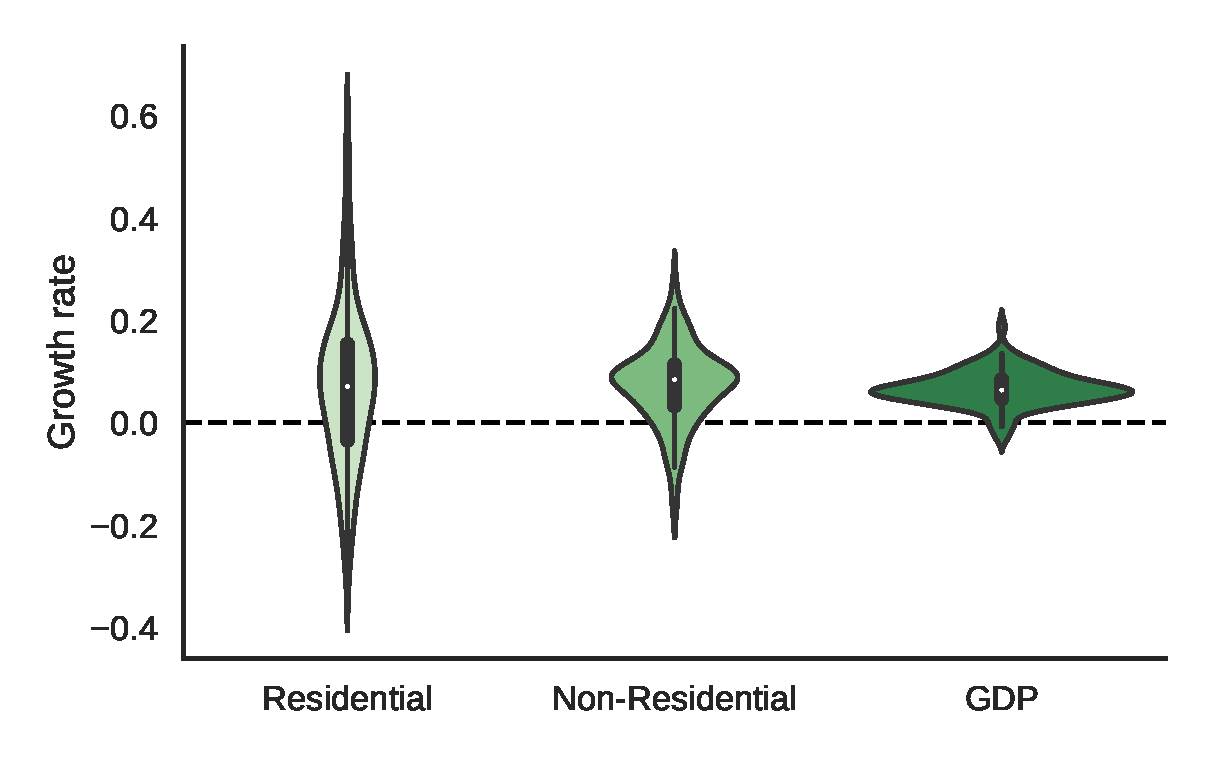
\includegraphics[width=.8\linewidth]{./figs/Volatilidade.eps}
	\end{subfigure}
	\begin{subfigure}[t]{.5\textwidth}
		\centering
		\caption{Autonomous expenditures share on GDP (US, 1979-2019)}
		\label{FigAutonomos}
		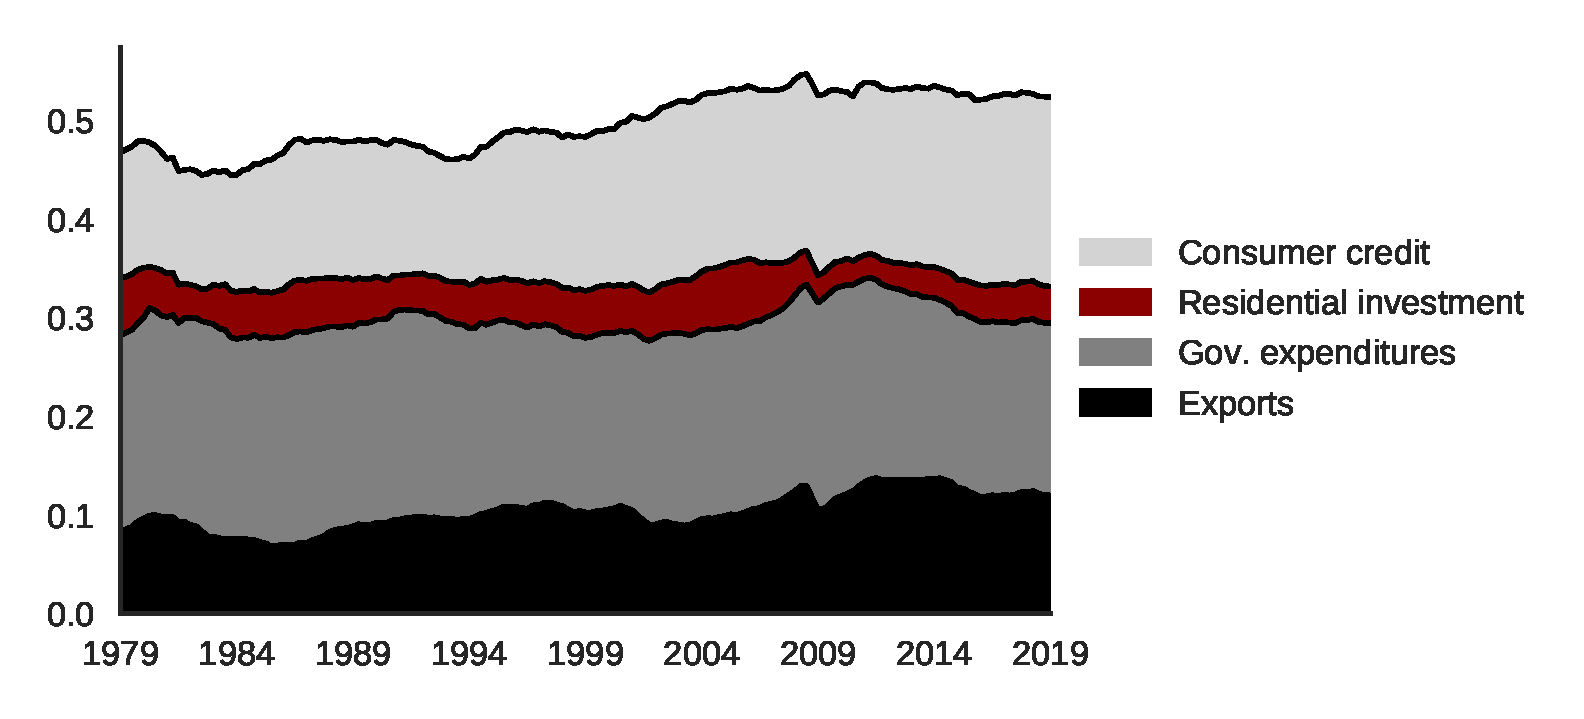
\includegraphics[width=.8\linewidth]{./figs/Gastos_autonomos.eps}  
	\end{subfigure}
	\caption*{\textbf{Source:} U.S. Bureau of Economic Analysis, Authors' Elaboration}
\end{figure}


It is worth mentioning the novelty of \textcite{green_follow_1997} and \textcite{leamer_housing_2007} --- revisited in \textcite{leamer_housing_2015} and by \textcite{fiebiger_trend_2017} --- when shedding light on the relevance of residential investment even before of the Great Recession.
More precisely, \textcite{green_follow_1997} reports that residential investment leads --- more than firms' investment --- the business cycle.
However, argues that this result does not imply a causal relationship:

\begin{quotation}
	[P]erhaps residential investment, like stock prices and interest rates, is a good predictor of GDP because it is a series that reflects \textbf{forward-looking behavior}. Presumably households will not increase their expenditures on housing unless they expect to prosper in the future. Building a house is a natural mechanism for doing this. Thus, the series can do a good job of predicting GDP \textbf{without necessarily causing GDP} (\cite[p.~267, ephasis added]{green_follow_1997}).
\end{quotation}
Despite paying attention to non-capacity creating autonomous expenditure, \textcite{green_follow_1997}, restricts its relevance as temporal precedence indicator.
\textcite{leamer_housing_2007}, on the other hand, reports a causal relationship between housing and GDP.
In summary, states that residential investment implies a higher durable goods consumption, that is, the US business cycle is a ``consumer cycle''.

Next, we present Figure \ref{FigIh_u} in order to depict the relation between housing and business cycle in which each cycle is represented in a different panel\footnote{FIEBIGER}. 
The vertical axis represents residential investment-GDP ratio and the horizontal
axis represents the rate of capacity utilization as a proxy for business cycle.
Economic recovery is generally characterized residential investment growing faster than GDP --- with the 1991-2000 period being a particular case. 
As a consequence of this higher growth rate, is the increase of both residential investment share on GDP and capacity utilization. 
Following the Sraffian supermultiplier growth model, we conclude that increase of non-residential investment is the result of capital stock adjustment principle.
This increase implies GDP to grow faster than residential investment, therefore reducing both its share on GDP and capacity utilization ratio. 
Finally, as a result of economic burst, capacity utilization ratio falls and the cycle.


\begin{figure}[H]
	\centering
	\caption{Residential investment share on GDP VS. capacity utilization during recessions}
	\label{FigIh_u}
	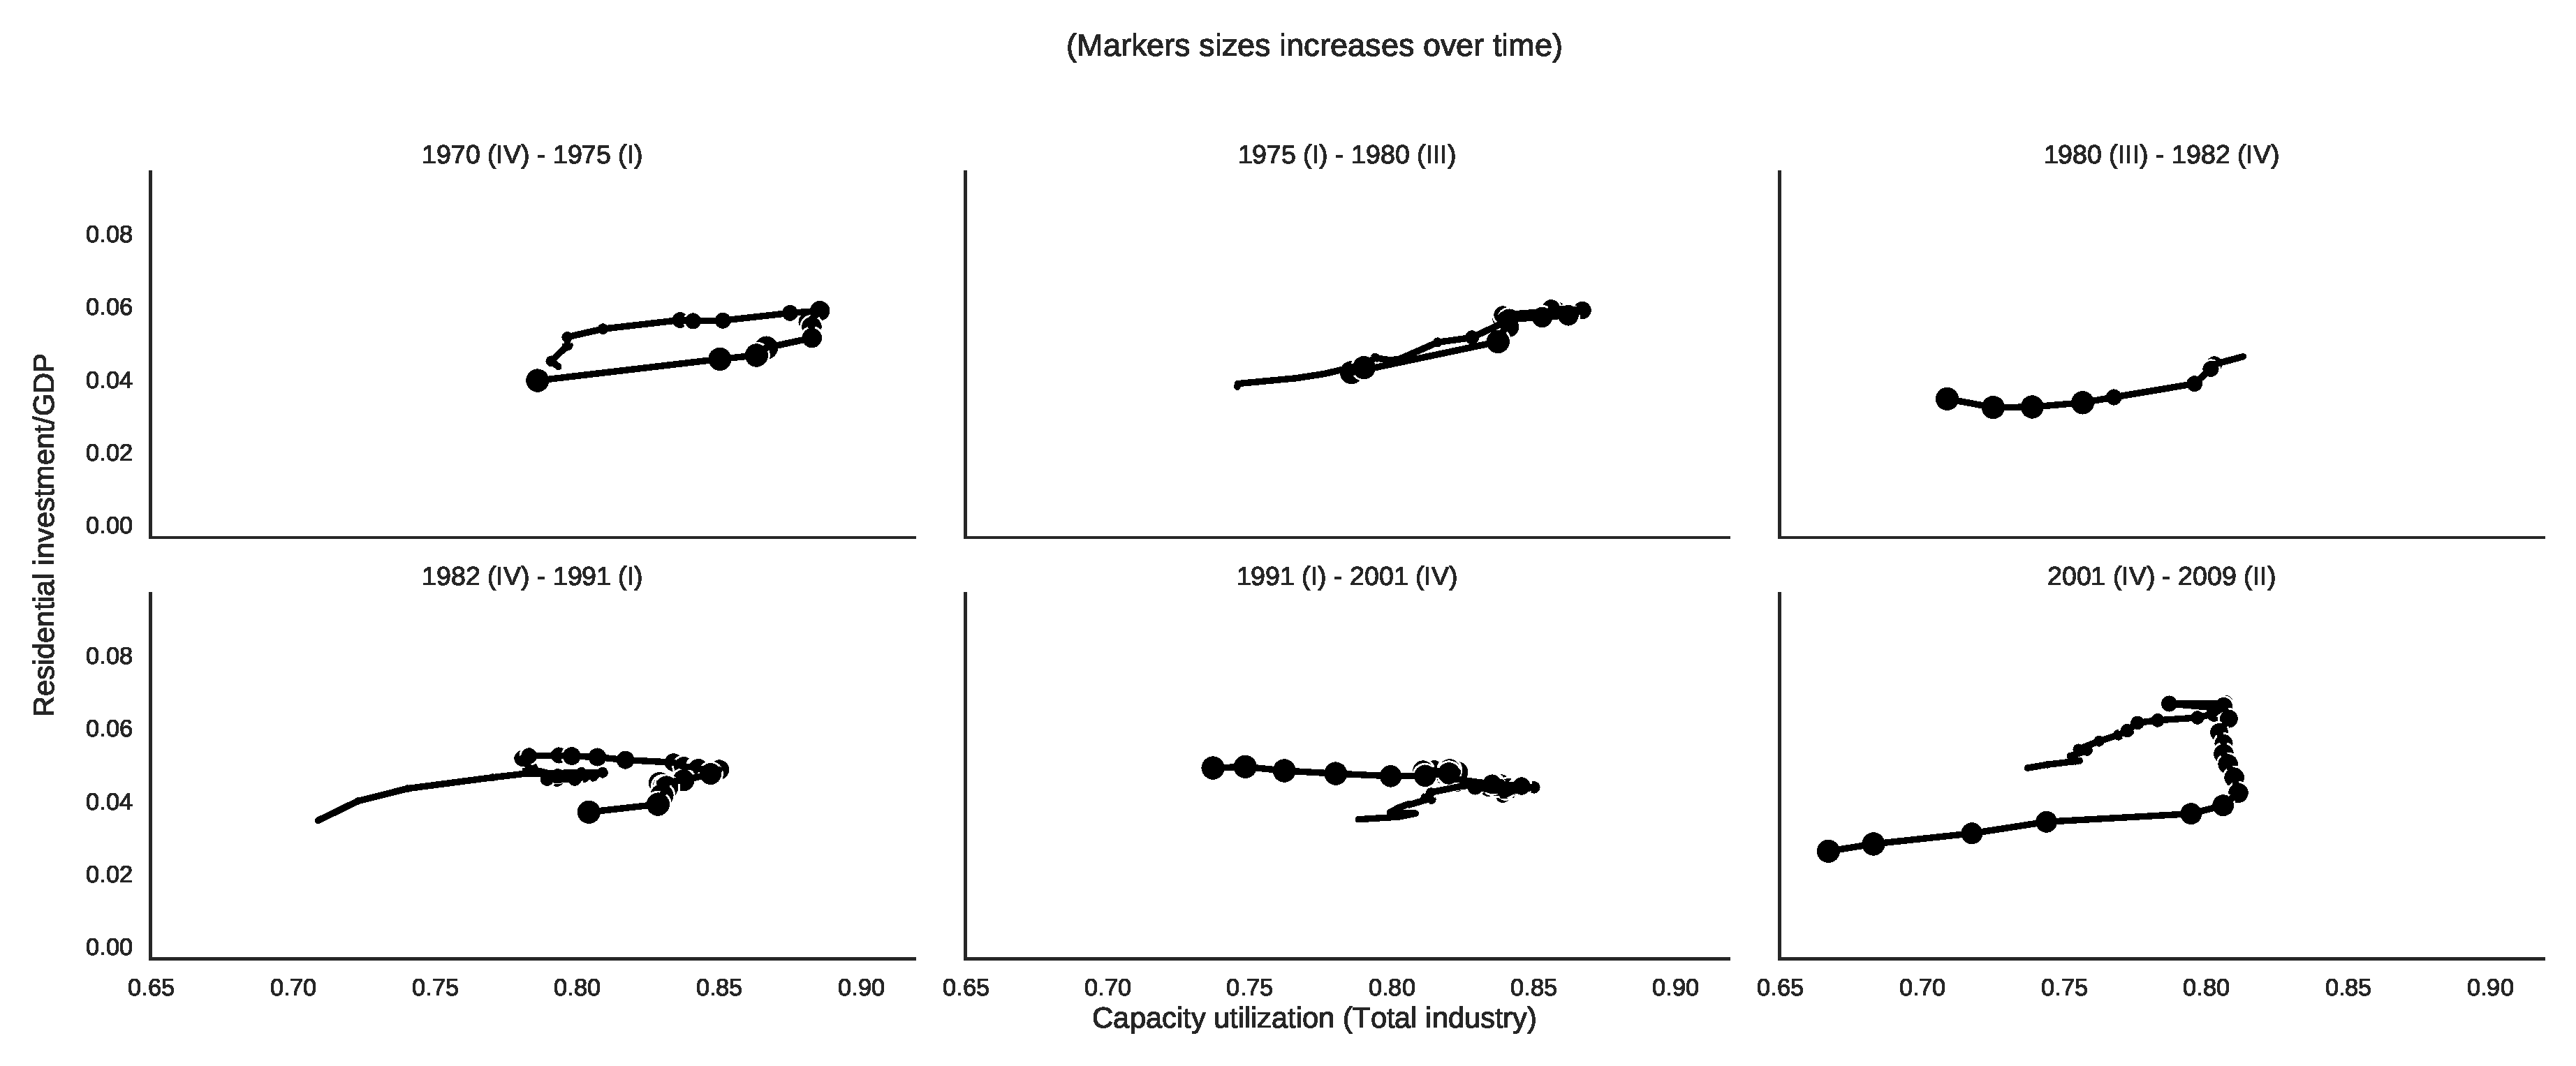
\includegraphics[width=\textwidth]{./figs/Ciclo_Ih_u.eps}
	\caption*{\textbf{Source:} Authors' Elaboration}
\end{figure}

There is also an indirect relation between housing and aggregate demand. 
Real estate constitutes a significant portion of household wealth so houses serves as collateral to borrowing (\cite{teixeira_uma_2011}). 
As a consequence of US institutional arrangement, households --- especially the poorest ones --- could increase their indebtedness as houses prices went up (see Figure \ref{FigDividaPreco}) as a way to ``realize'' capital gains without
selling their homes during house bubble of the 2000s (\cite{teixeira_crescimento_2015}).
Therefore, real estate inflation and durable goods consumption are connected and has relevant consequences for business cycle.
\textcite{zezza_u.s._2008} and \textcite{barba_rising_2009}, for example, report that credit-financed consumption was one of the main drivers of economic growth before the Great Recession.




\begin{figure}[H]
	\centering
	\caption{Household indebtedness and house prices dynamics (jan/2000=100)}
	\label{FigDividaPreco}
	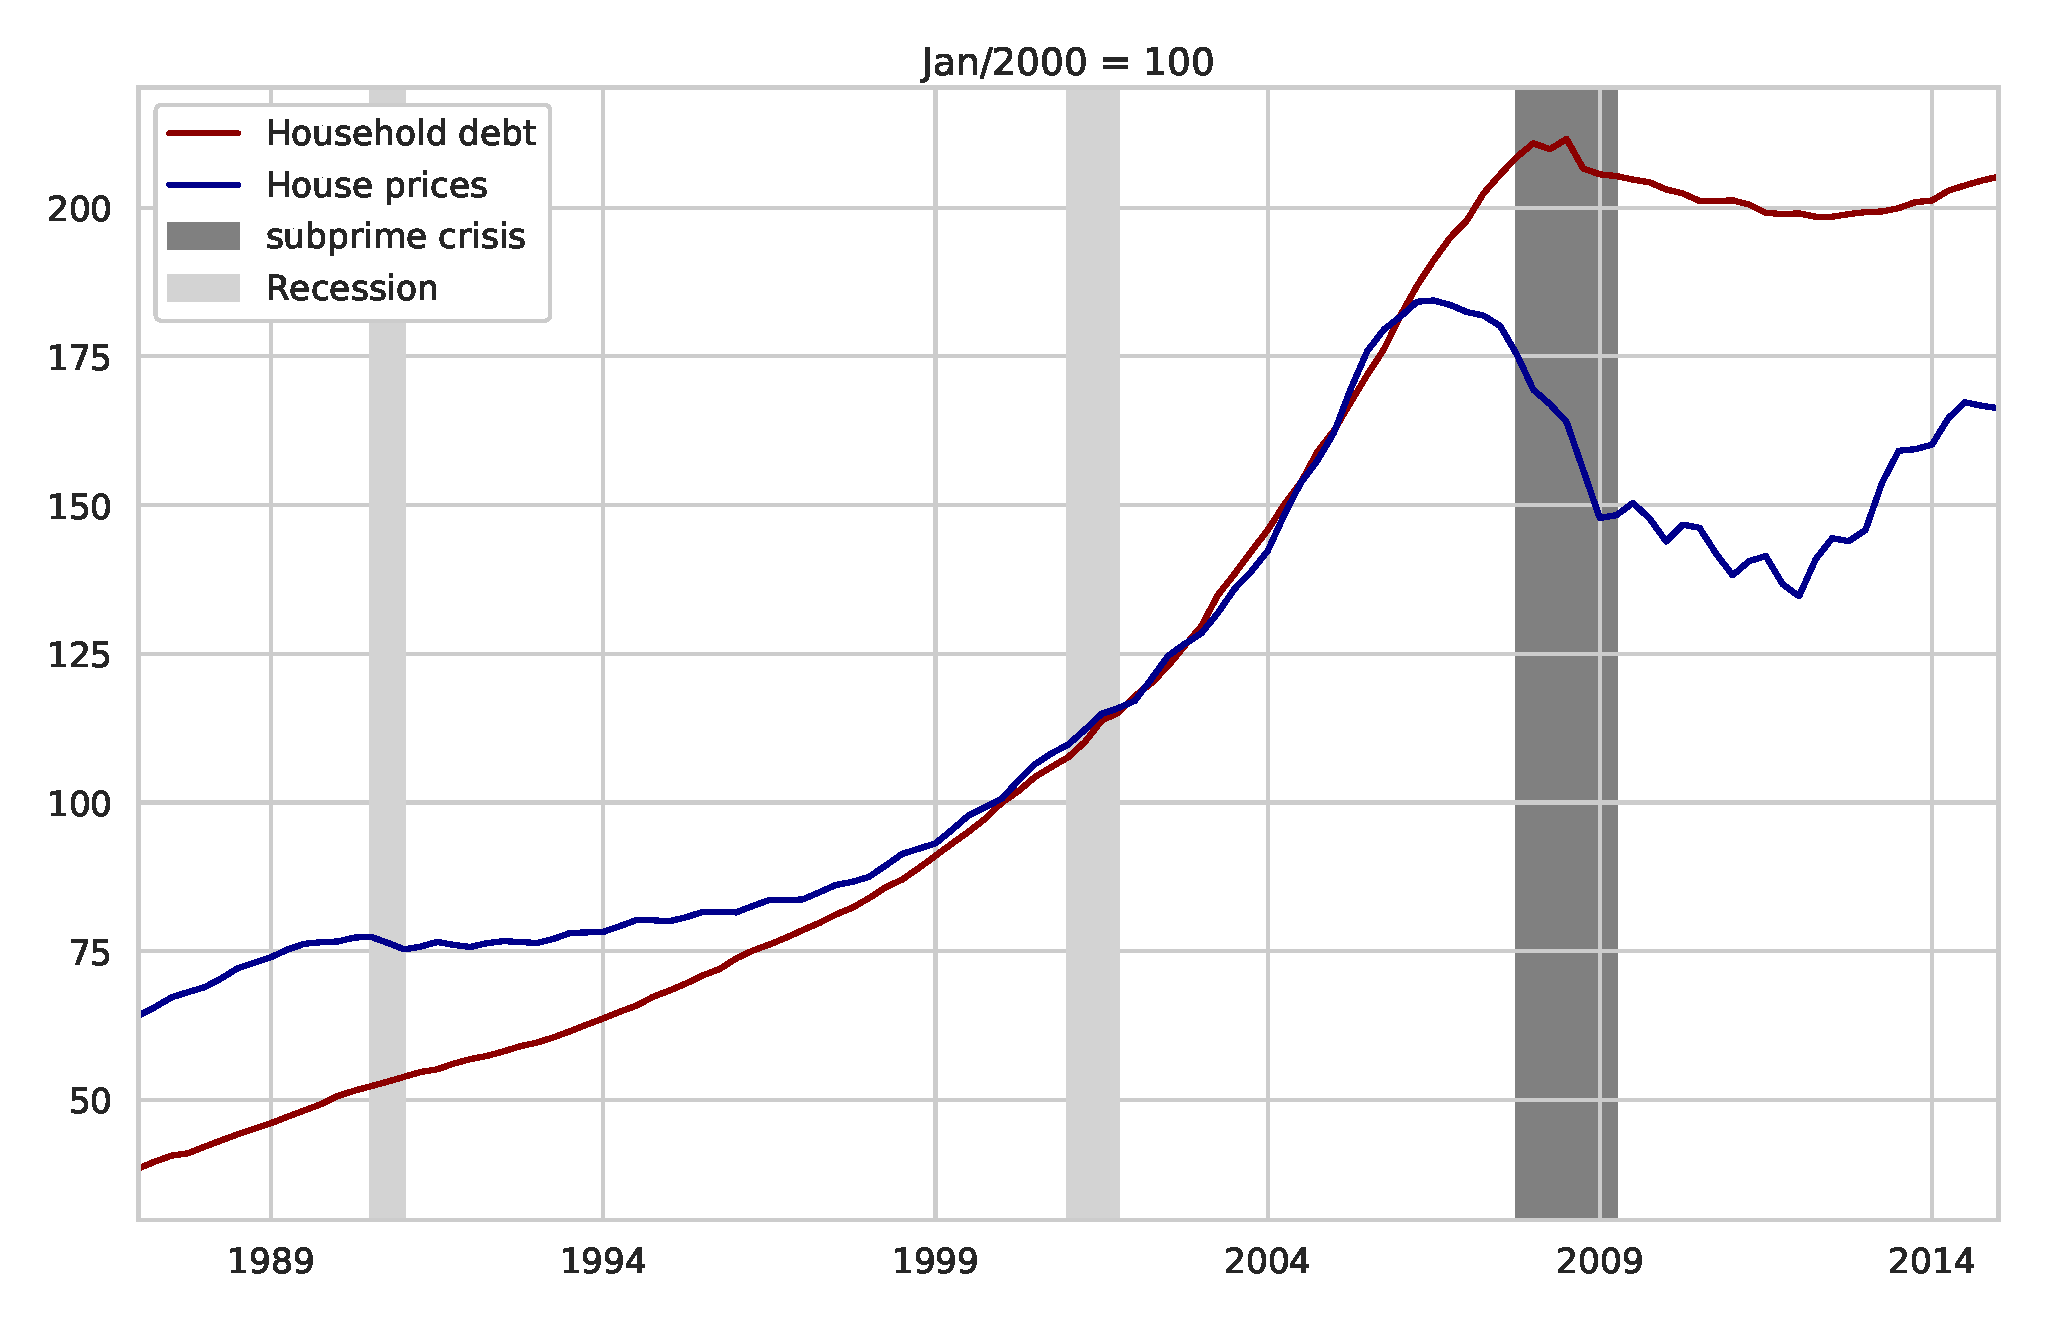
\includegraphics[width=\textwidth]{./figs/Divida_PrecoImoveis.eps}
	\caption*{\textbf{Source:} U.S. Bureau of Economic Analysis, Authors' Elaboration}
\end{figure}
This relation between households indebtedness and real estate inflation has other relevant implications.
The first is the gap between assets and liabilities in the course of the Great Recession.
This dynamic is due both to the housing prices burst (post-2005) and to the insensitivity of households' financial commitments.
In other words, real estate (assets) has a market value while debt (liabilities) has a contractual one, thus, households net worth decreases onset of the subprime crisis.
Therefore, the second implication is the sharp reduction in the net worth of the poorest households in absolute and relative terms (see Figure \ref{FigDistPassivos}).


\begin{figure}
	\centering
	\caption{Liabilities evolution by wealth percentile (1989/07=1)}
	\label{FigDistPassivos}
	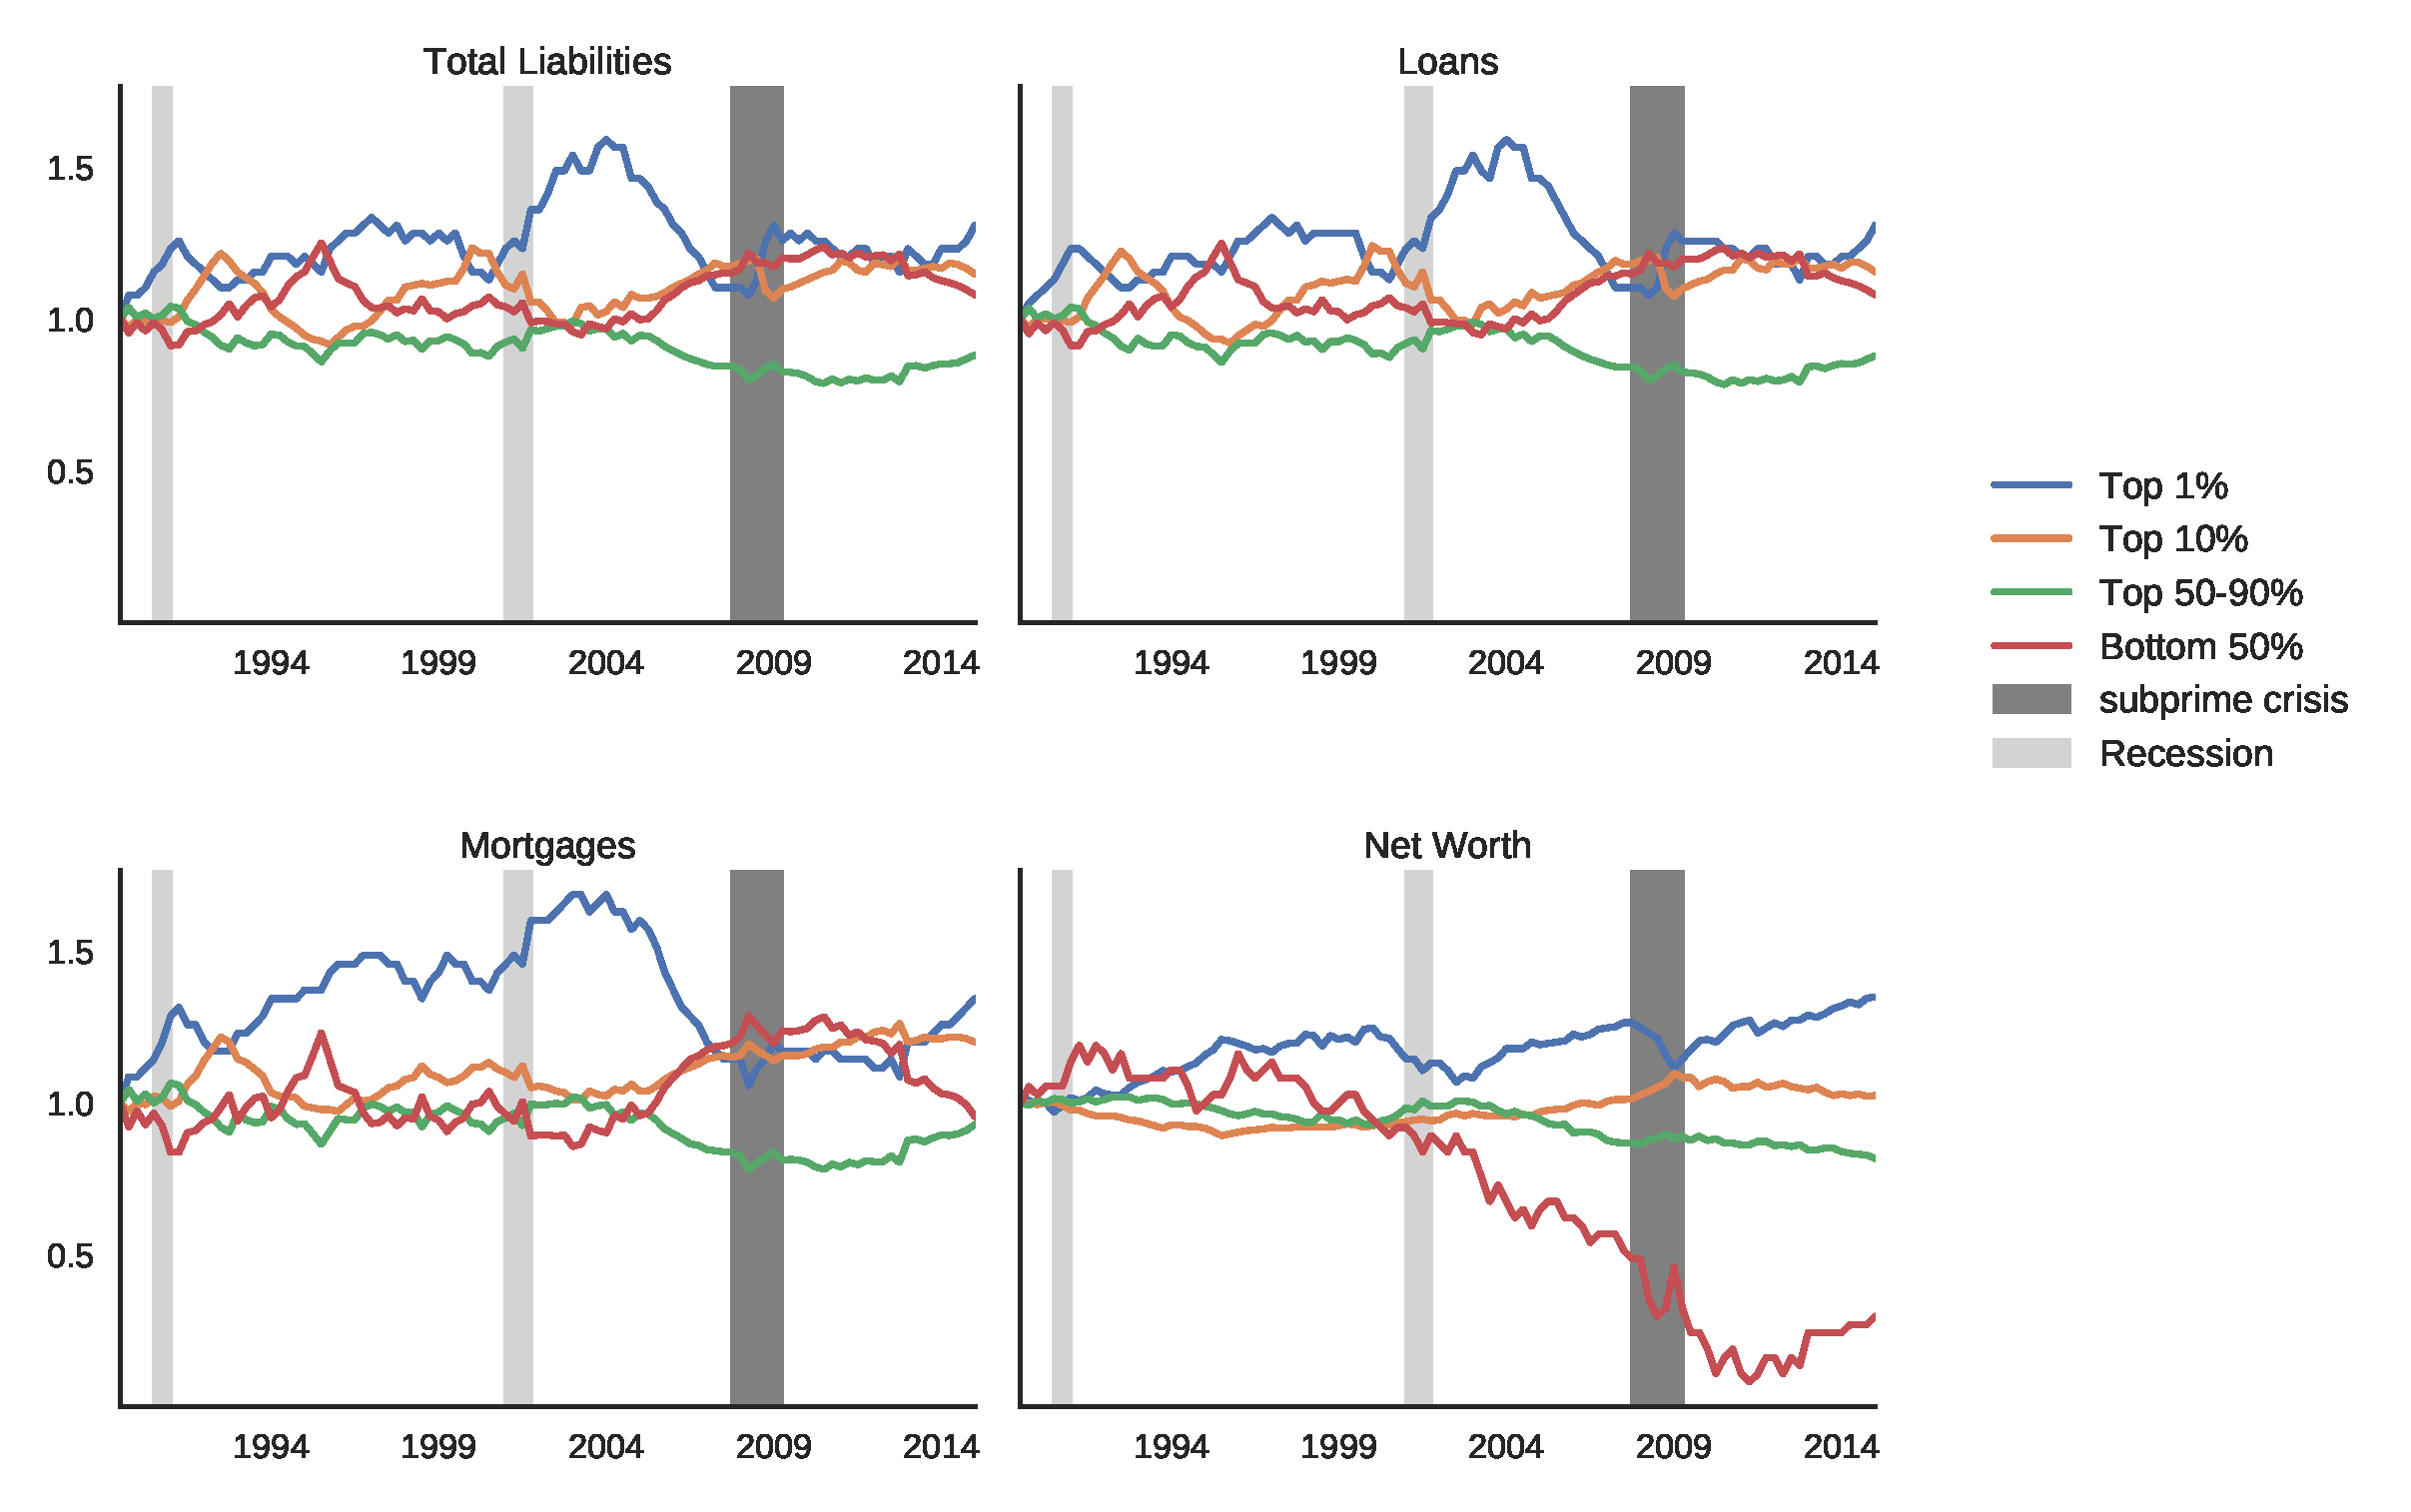
\includegraphics[width=.8\textwidth]{./figs/Distribuicao_Passivos.eps}
	\caption*{\textbf{Source:} \textcite{us_census_bureau_characteristics_2017}, Authors' Elaboration}
\end{figure}

In summary, we conclude that housing is relevant to understand the specificity of US business cycle.
On the following section, we analyze how econometric literature has dealt with the topic.
More precisely, we evaluate macroeconometric works according to its compatibility with Sraffian supermultiplier growth model.

\section{Review of the Macroeconometric Literature}\label{sec:empirical_review}


It worth noting that most papers that includes residential investment has failed to treat it macroeconomically, restricting it to microeconomic and regional issues (\cite{arestis_u.s._2008}).
However, after the burst of the US housing bubble, there have been a growing attention in the macroeconomic implications of residential investment.
In this context, we analyze the macroeconometric literature that explicitly includes housing to evaluate the determinants of its growth rate.
Each model will be analyzed according to the compatibility with demand-led growth agenda as well as the possibility of including asset bubbles.

In this sense, \textcite{poterba_tax_1984} contribution stands out once it does not assume instantly convergence of real estate supply to the desired level.
Furthermore, this theoretical frame considers residential investment as induced positively by house prices.
Despite the novelty, this work does not include asset bubbles.
In this context,  \textcite{arestis_residential_2015} update \textcite{poterba_tax_1984} framework by estimating an autoregressive distributed lag (ARDL) model for 17 OECD countries.
In summary, they conclude that residential investment depends mainly on disposable income.
This result would  question the possibility of treating housing as an autonomous expenditure and jeopardize the analysis from the Sraffian supermultiplier perspective.
However, the authors themselves find that this result is not statistically significant for the US in which real house prices and the volume of banking credit are the main determinant of residential investment.
In this sense, this result allows considering housing as a non-capacity creating autonomous expenditure.

Alternatively, \textcite{huang_is_2018} assess both \textcite{leamer_housing_2007} hypotheses related to residential investment (prediction and causality). 
To do so, they estimate a Structural Vector Autoregressive (SVEC) model with wavelets transformation for some OECD countries
They find residential investment is not only as monetary policy transmission channel, but it also has temporally distinct effects on business cycle.
In the short-run, housing is more predictive while house prices have a bigger influence in the long-run\footnote{
	More precisely, \textcite{huang_is_2018} also conclude that residential investment prediction increases with its share on GDP.
}. 
These distinct temporal influence of housing occurs due to the large wealth effect in the long-run while credit and collateral effect are more relevant in the short-run.
Regarding the causal relationship described by \textcite{leamer_housing_2007}, 
\textcite{huang_is_2018} report inconclusive results for all countries due to their institutional heterogeneity\footnote{
	However, \textcite{huang_is_2018} claim that for most G7 countries, residential investment at least amplify the business cycle.
}, but remains valid for the US.
Despite the inconclusive results on fluctuations, they find that the variables associated with residential investment (house prices, real mortgage rate --- deflated by a general price index --- and bank spread) lead the business cycle.

Despite clarifying some macroeconomics  implications of housing on the business cycle, the results reported above are centered on supply side variables.
\textcite{gauger_residential_2003}, on the other hand, evaluate the consequences of deregulation of depository institutions throughout the 1980s.
To do so, they estimate a VECM between monetary aggregates (M2), GDP, residential investment and alternate between short-term government bonds and long-term mortgage interest rates. 
They report an increasing contribution of long-term mortgages interest rate over resident investment variance after those institutional chances mentioned above:

\begin{quotation}
	The findings for the two interest rates give valuable information to evaluate results in other studies. Results here suggest that use of a short-term FFR and post-deregulation data may lead to conclusions that `interest rate shocks are much less important after deregulation.' The fuller state of evidence here indicates that interest rate shocks remain important post-deregulation; however, now it is the long-term rate shocks that carry more information for housing sector movements (\cite[p.~346]{gauger_residential_2003})
\end{quotation}
It worth noting that \textcite{gauger_residential_2003} work reports other two interesting results:
	(i) GDP level is determined --- as Sraffian supermultiplier  suggests --- by residential investment and both expenditures share a common long-term trend;
	(ii) show some relevant institutional changes in real estate market.

Figure \ref{Fig:CreditFDICIA} illustrates item (ii) mentioned above in which we mark some reforms that occurred due to the savings and loans crisis throughout the 80's and early 90's.
This institutional changes --- notably Financial Institutions Reform, Recovery, and Enforcement Act (FIRREA) in 1989 and Federal Deposit Insurance Corporation Improvement Act  (FDICIA) in 1991 --- increased the credit volume to households\footnote{
	\textcite{federal_deposit_insurance_corporation_savings_1997} argues that this consequence stems from the different regulation of S\&L compared to commercial banks. The financial deregulation of the 1980s encouraged speculation in other sectors, especially real estate. As a consequence, engendered a banking run, increasing overall credit volume, which, however, was followed by the S\&L crisis:
	\begin{quotation}
		Clearly, competition from savings and loans did not cause the various crises experienced by the commercial banking industry during the 1980s; these crises would have occurred regardless of the thrift situation. But the channeling of large volumes of deposits into high-risk institutions that speculated in real estate development did create marketplace distortions (\cite[p.~168]{federal_deposit_insurance_corporation_savings_1997})
	\end{quotation}
	Therefore, the increase in credit volume cannot be dissociated from speculation with real estate.
}\footnote{
	According to \textcite{federal_deposit_insurance_corporation_savings_1997}, had two main objectives:
		(i) Recapitalize the bank insurance fund and;
		(ii) Reform the deposit guarantee system and bank regulation to minimize  taxpayer in the event of bank collapse (\cite{mishkin_evaluating_1997}).
		\textcite[p.~170]{federal_deposit_insurance_corporation_savings_1997} describe banking operation before FDICIA as follows:
		\begin{quotation}
			Legislation for S\&Ls was driven by the public policy goal of encouraging home ownership. It began with the Federal Home Loan Bank Act of 1932, which established the Federal Home Loan Bank System as a source of liquidity and low-cost financing for S\&Ls.
		\end{quotation}
	and the implications after its implementation is depicted as:
		\begin{quotation}
			Prior to the act’s passage, the FDIC and the Federal Savings and Loan Insurance Corporation provided 100 percent \textit{de facto} deposit insurance at almost all failed banks. The FDIC did so by comparing bids to acquire the entire bank (including all its deposits) with the cost of liquidating the bank, which generally produced the result that covering all deposits was less expensive (FDIC 2003, chap. 2). FDICIA sought to change this process by mandating least-cost resolution, which required consideration of all possible resolution methods (FDIC 2003, chap. 2) (\cite[p.~iii]{wall_too_2010})
		\end{quotation}
		
}. As a consequence, real estate finance has increased considerably in the following periods.

\begin{figure}[htb]
	\centering
	\caption{Mortgage and Consumer credit growth rate (1979-2019)}
	\label{Fig:CreditFDICIA}
	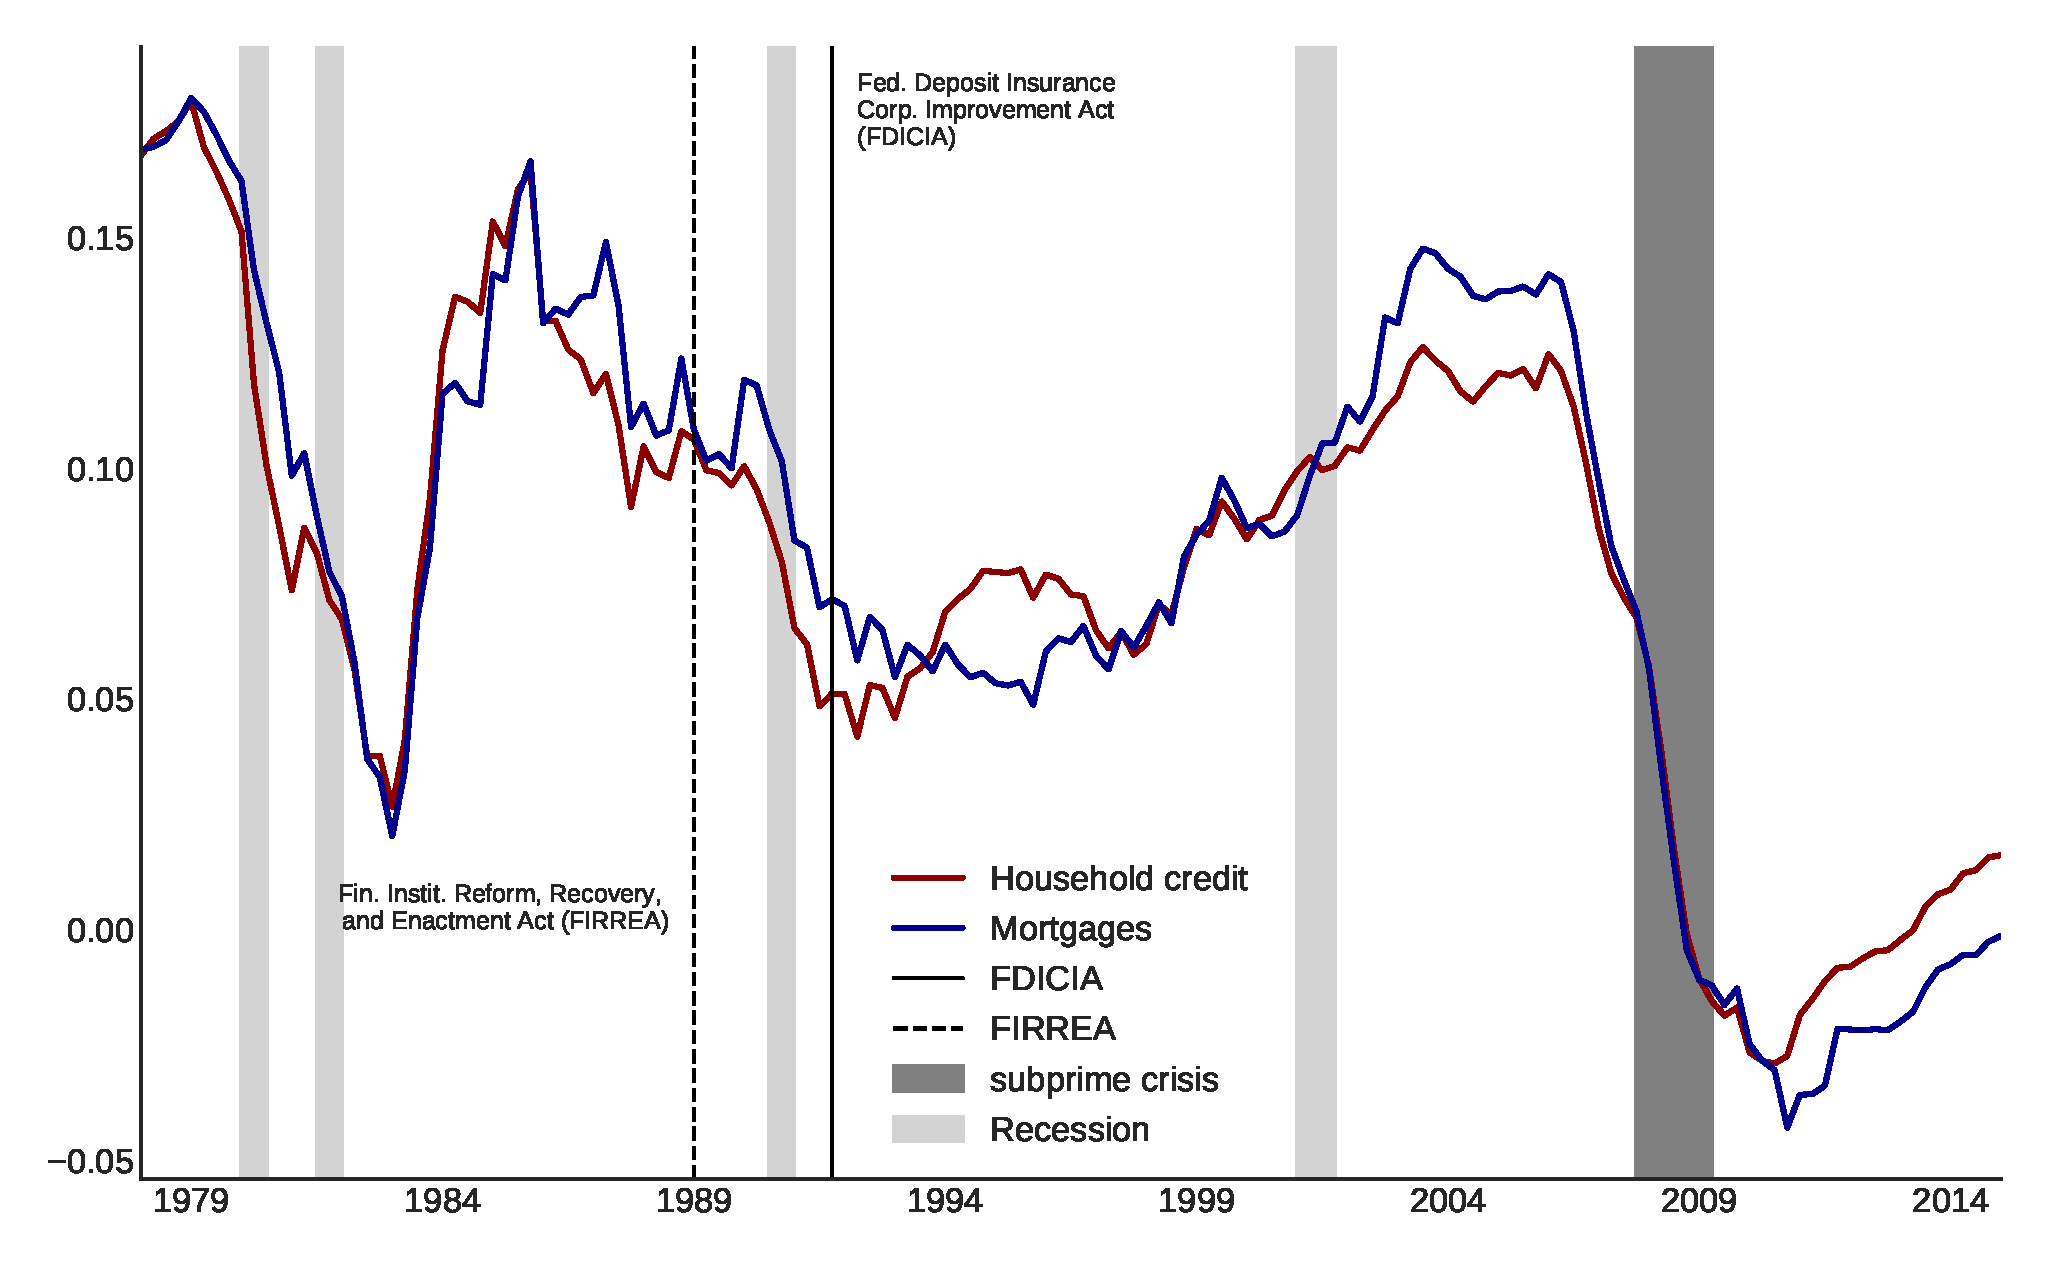
\includegraphics[width=\textwidth]{./figs/FDICIA.eps}
	\caption*{\textbf{Source:} U.S. Bureau of Economic Analisys, Authors' elaboration}
\end{figure}
Although \textcite{gauger_residential_2003} emphasize the relevance of long-term mortgages interest rate in residential investment dynamics, this procedure is not appropriate once policy rate is determined by monetary aggregates.
Thus, such a proposal is incompatible with modern macroeconomic theory in which policy rate is an exogenous variable determined through a decision-making process (\cite[p.~230--256]{lavoie_post-keynesian_2015}).

One way to include residential investment in demand-led growth agenda without incurring problems mentioned above is the houses' own interest rate proposed by \textcite{teixeira_crescimento_2015}.
In summary, this particular real interest rate depicts both debt service and capital gains effects in households' net worth.
On the following section, we discuss this proposal in further details and then evaluate its relevance in a macroeconometric model.


\section{Modelo macroeconométrico}
\label{Modelo_empirico}

O modelo a ser estimado pretende testar se a inflação de ativos (\textit{i.e.} inflação do preço dos imóveis) contribui para explicar a dinâmica do investimento residencial tal como proposto por \textcite{teixeira_crescimento_2015}. 
Vale relembrar que a seleção do período analisado decorre de quebras estruturais (ver tabela \ref{structbreak}) associadas às mudanças institucionais no-pós crise dos \textit{savings and loans} (FDIC e FIRREA).
Dito isso, foram utilizadas séries trimestrais com ajuste sazonal de 1992 a 2019 (ver gráfico \ref{YeoJhonson}) da taxa de juros das hipotecas fixas em trinta anos (MORTGAGE30US, trimestralizada pelo fim do período), investimento residencial (PRFI, em taxa de crescimento) e índice de Case-Shiller (CSUSHPISA, trimestralizada pelo fim do período). 

Por se tratar de taxas de crescimento com ampla volatilidade, aplicou-se a transformação de \textcite{yeo_new_2000} para conter a amplitude das séries decorrente da crise imobiliária. A razão de se utilizar tal procedimento e não a transformação de \textcite{box_analysis_1964} é por não se restringir a valores não-negativos. Em seguida, foram realizados testes de raiz unitária (tabela \ref{unitroot}) bem como o procedimento de \textcite{johansen_estimation_1991} (tabela \ref{Johansen}) e, a um nível de significância de 5\%, conclui-se que as séries são cointegradas e, portanto, um modelo do tipo vetor de correção de erros (VECM) é a melhor forma de estimação para este caso \cite{enders_applied_2014}.


%TODO Alterar figura
\begin{figure}[H]
	\centering
	\caption{Séries com transformação de \textcite{yeo_new_2000}}
	\label{YeoJhonson}
	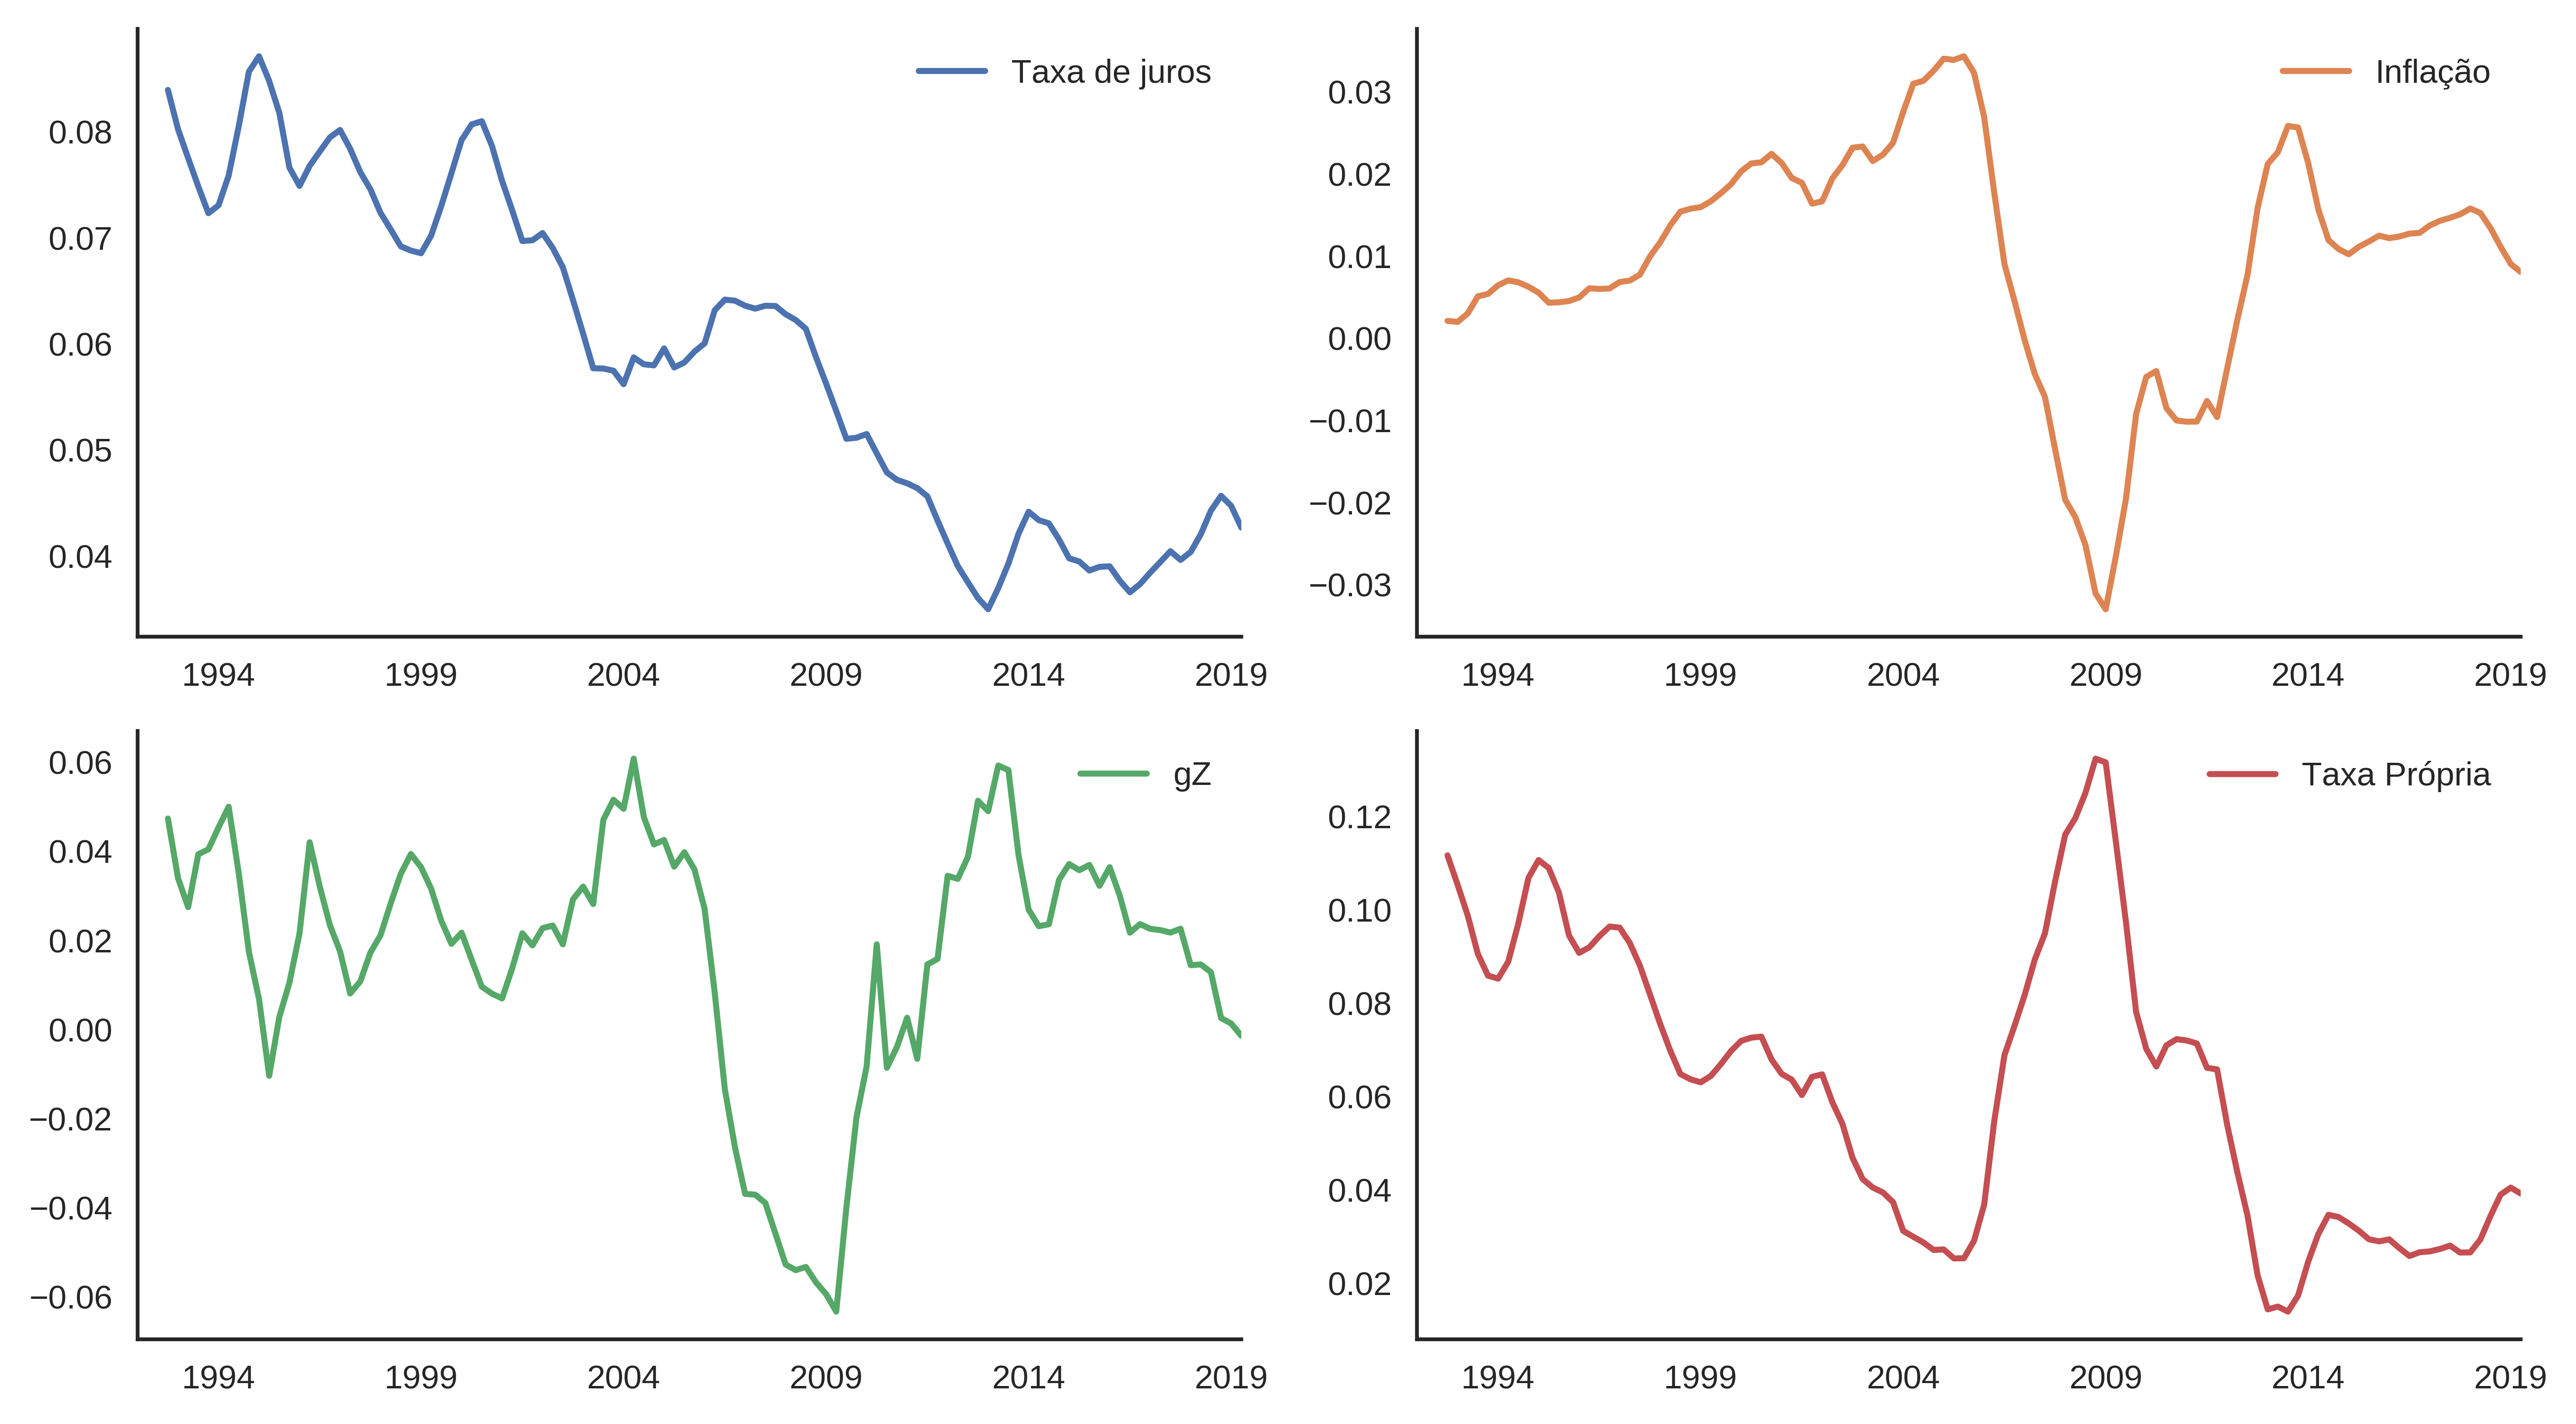
\includegraphics[width=\textwidth]{../../Dados/Fatos_Estilizados/figs/YeoJohnson_All.png}
	\caption*{\textbf{Fonte:} U.S. Bureau of Economic Analysis, elaboração própria}
\end{figure}


Dito isso, resta determinar a defasagem utilizada. Pelos critérios de informação, tanto o primeiro (trimestre) quanto o quarto \textit{lag} são elegíveis (ver tabela \ref{criterios}). Apesar de parcimonioso, a escolha da primeira defasagem não possui respaldo teórico e isso pode ser visualizado pelo gráfico \ref{meses}. Se considerar o tempo médio de construção de imóveis desde a aprovação até a conclusão, verifica-se que deve-se incluir \textit{ao menos} o segundo \textit{lag} para incorporar as residências construídas para a venda uma vez que tal motivação só é realizada se concluída a construção. Tal procedimento, no entanto, não é suficiente para determinar a seleção do \textit{lag} a ser utilizado. Dado que o fluxo de novos imóveis é significativamente inferior ao estoque existente, o efeito da variação dos preços se verifica mesmo com as construções não concluídas, ou seja, impacto decorre das residências concluídas anteriormente.  Tal elemento seria captado pela taxa própria \textit{esperada}. No entanto, não há uma série para tal de modo que as defasagens são uma primeira aproximação para a taxa esperada.


\begin{table}[htb]
	\caption{Seleção da ordem do VECM (* indica o mínimo)}
	\label{criterios}
\begin{center}
\begin{tabular}{lcccc}
\toprule
            & \textbf{AIC} & \textbf{BIC} & \textbf{FPE} & \textbf{HQIC}  \\
\midrule
\textbf{0}  &      -14.96  &     -14.69*  &   3.186e-07  &      -14.85*   \\
\textbf{1}  &      -14.99  &      -14.61  &   3.100e-07  &       -14.83   \\
\textbf{2}  &      -14.96  &      -14.47  &   3.196e-07  &       -14.76   \\
\textbf{3}  &      -14.98  &      -14.39  &   3.112e-07  &       -14.74   \\
\textbf{4}  &      -15.09  &      -14.39  &   2.806e-07  &       -14.81   \\
\textbf{5}  &      -15.09  &      -14.28  &   2.802e-07  &       -14.77   \\
\textbf{6}  &     -15.12*  &      -14.20  &  2.735e-07*  &       -14.75   \\
\textbf{7}  &      -15.09  &      -14.06  &   2.840e-07  &       -14.67   \\
\textbf{8}  &      -15.05  &      -13.92  &   2.948e-07  &       -14.59   \\
\textbf{9}  &      -14.98  &      -13.73  &   3.188e-07  &       -14.48   \\
\textbf{10} &      -14.97  &      -13.62  &   3.238e-07  &       -14.42   \\
\textbf{11} &      -14.94  &      -13.48  &   3.358e-07  &       -14.35   \\
\textbf{12} &      -14.88  &      -13.31  &   3.603e-07  &       -14.24   \\
\textbf{13} &      -14.91  &      -13.24  &   3.511e-07  &       -14.24   \\
\textbf{14} &      -14.86  &      -13.07  &   3.763e-07  &       -14.13   \\
\textbf{15} &      -14.82  &      -12.93  &   3.934e-07  &       -14.06   \\
\bottomrule
\end{tabular}
%\caption{VECM Order Selection (* highlights the minimums)}
\end{center}
\caption*{\textbf{Fonte:} Elaboração própria}
\end{table}


\begin{figure}[H]
	\centering
	\caption{Tempo médio de construção (aprovação a conclusão) de imóveis para uma unidade familiar por propósito de construção exceto casas pré-fabricadas (1976-2018)}
	\label{meses}
	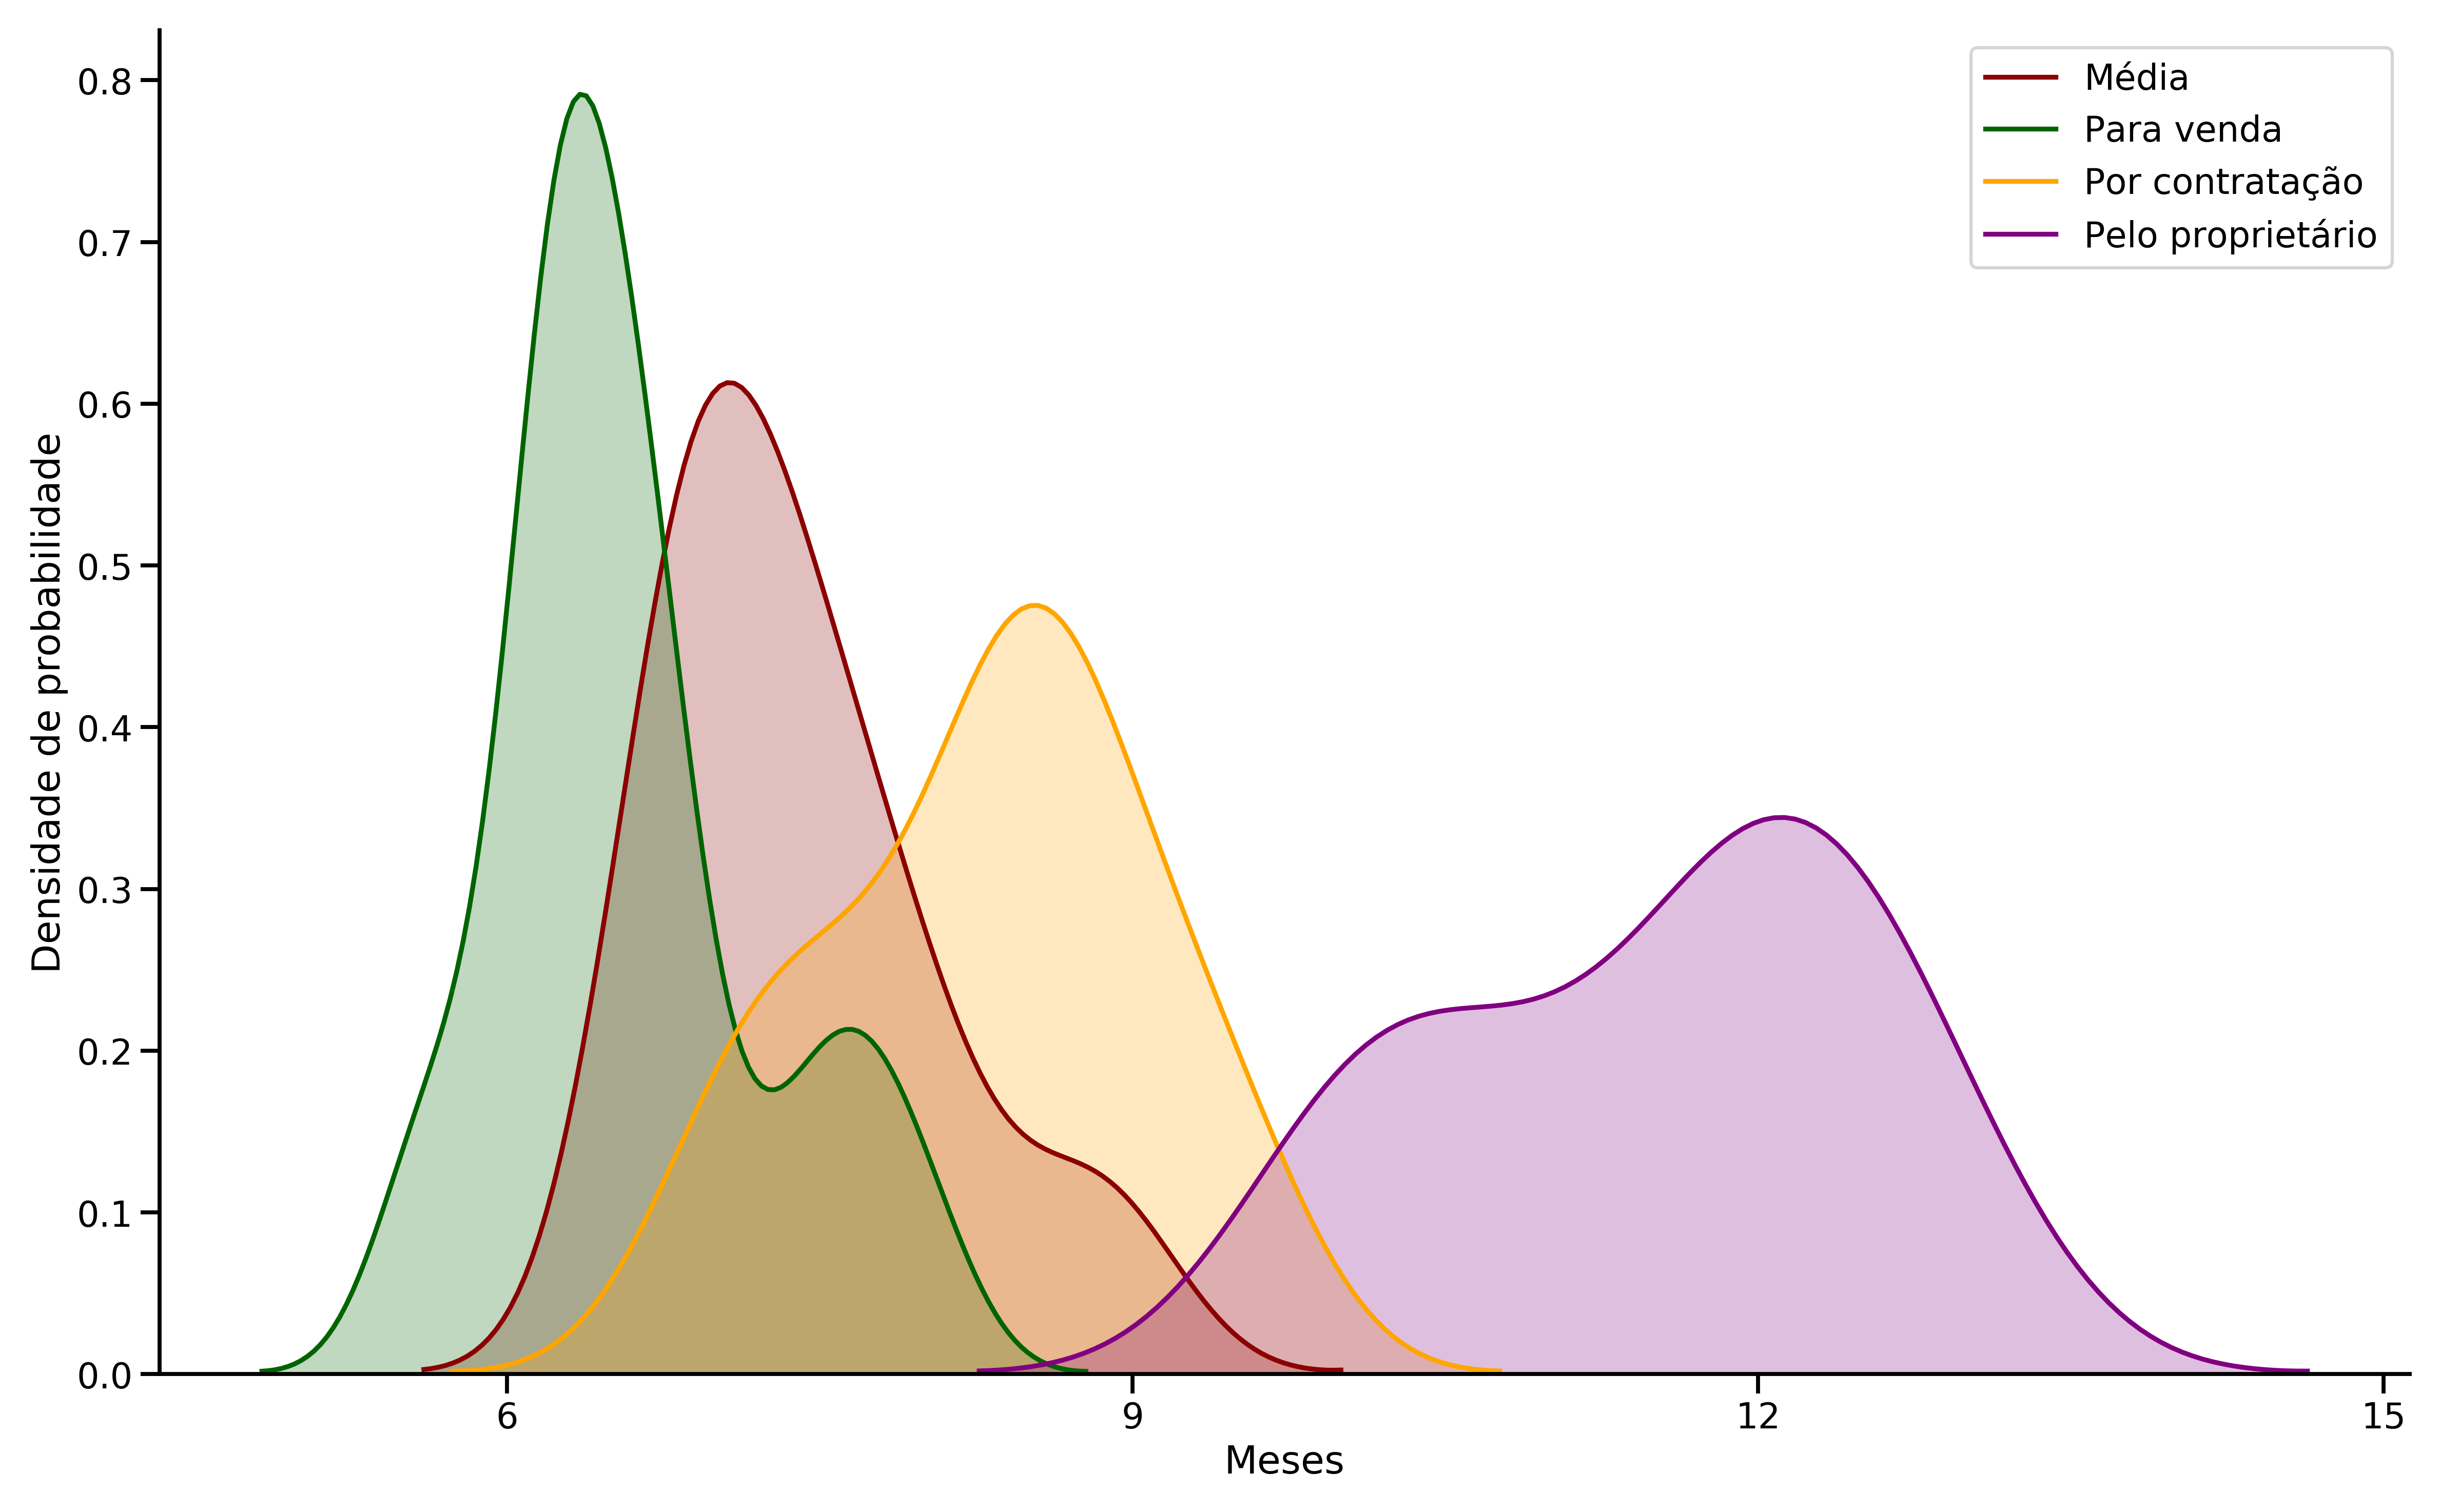
\includegraphics[width=\textwidth]{Fatos_Estilizados/Figs/Meses_contrucao.png}
	\caption*{\textbf{Fonte:} Survey of Construction (SOC), elaboração própria}
\end{figure}

Desse modo, uma alternativa é por meio de uma ``teoria prática do futuro'' --- como em \textcite[p.~214]{keynes_general_1937} --- em que o processo decisório para iniciar a construção de um novo imóvel depende de componentes expectacionais/convenções associados as observações passadas.
De forma a ilustrar tal relação, o gráfico \ref{defasagens} apresenta as variáveis de interesse frente ao \textit{lag} que minimiza os critérios de informação. Esse procedimento permite visualizar se existe alguma relação entre a taxa própria esperada (taxa efetiva defasada) e taxa de crescimento do investimento residencial\footnote{De modo a dar conta de não-linearidades, é apresentada a regressão quadrática entre ambas as variáveis (e o mesmo foi realizado para o gráfico inverso).}. Já a relação inversa, qual seja, da taxa de crescimento para a taxa própria não se verifica uma vez que, como visto, o fluxo de novos imóveis é bastante inferior o estoque de imóveis existente e, portanto, é esperado que tal relação não esteja presente. Em outras palavras, a especulação com o \textit{estoque}  de imóveis gera inflação desses ativos que, por conseguinte, afeta a construção de novos imóveis (\textit{fluxo}) e não o inverso. Essa inspeção, portanto, ilustra de forma bastante grosseira tal componente expectacional por meio da menor dispersão entre os pontos no gráfico inferior direito\footnote{Raciocínio semelhante pode ser encontrado em \textcite{girardi_autonomous_2015}}.  


\begin{figure}[htb]
	\centering
	\caption{Dispersão entre taxa própria e crescimento do investimento residencial: defasagens selecionadas a partir dos critérios de informação}
	\label{defasagens}
	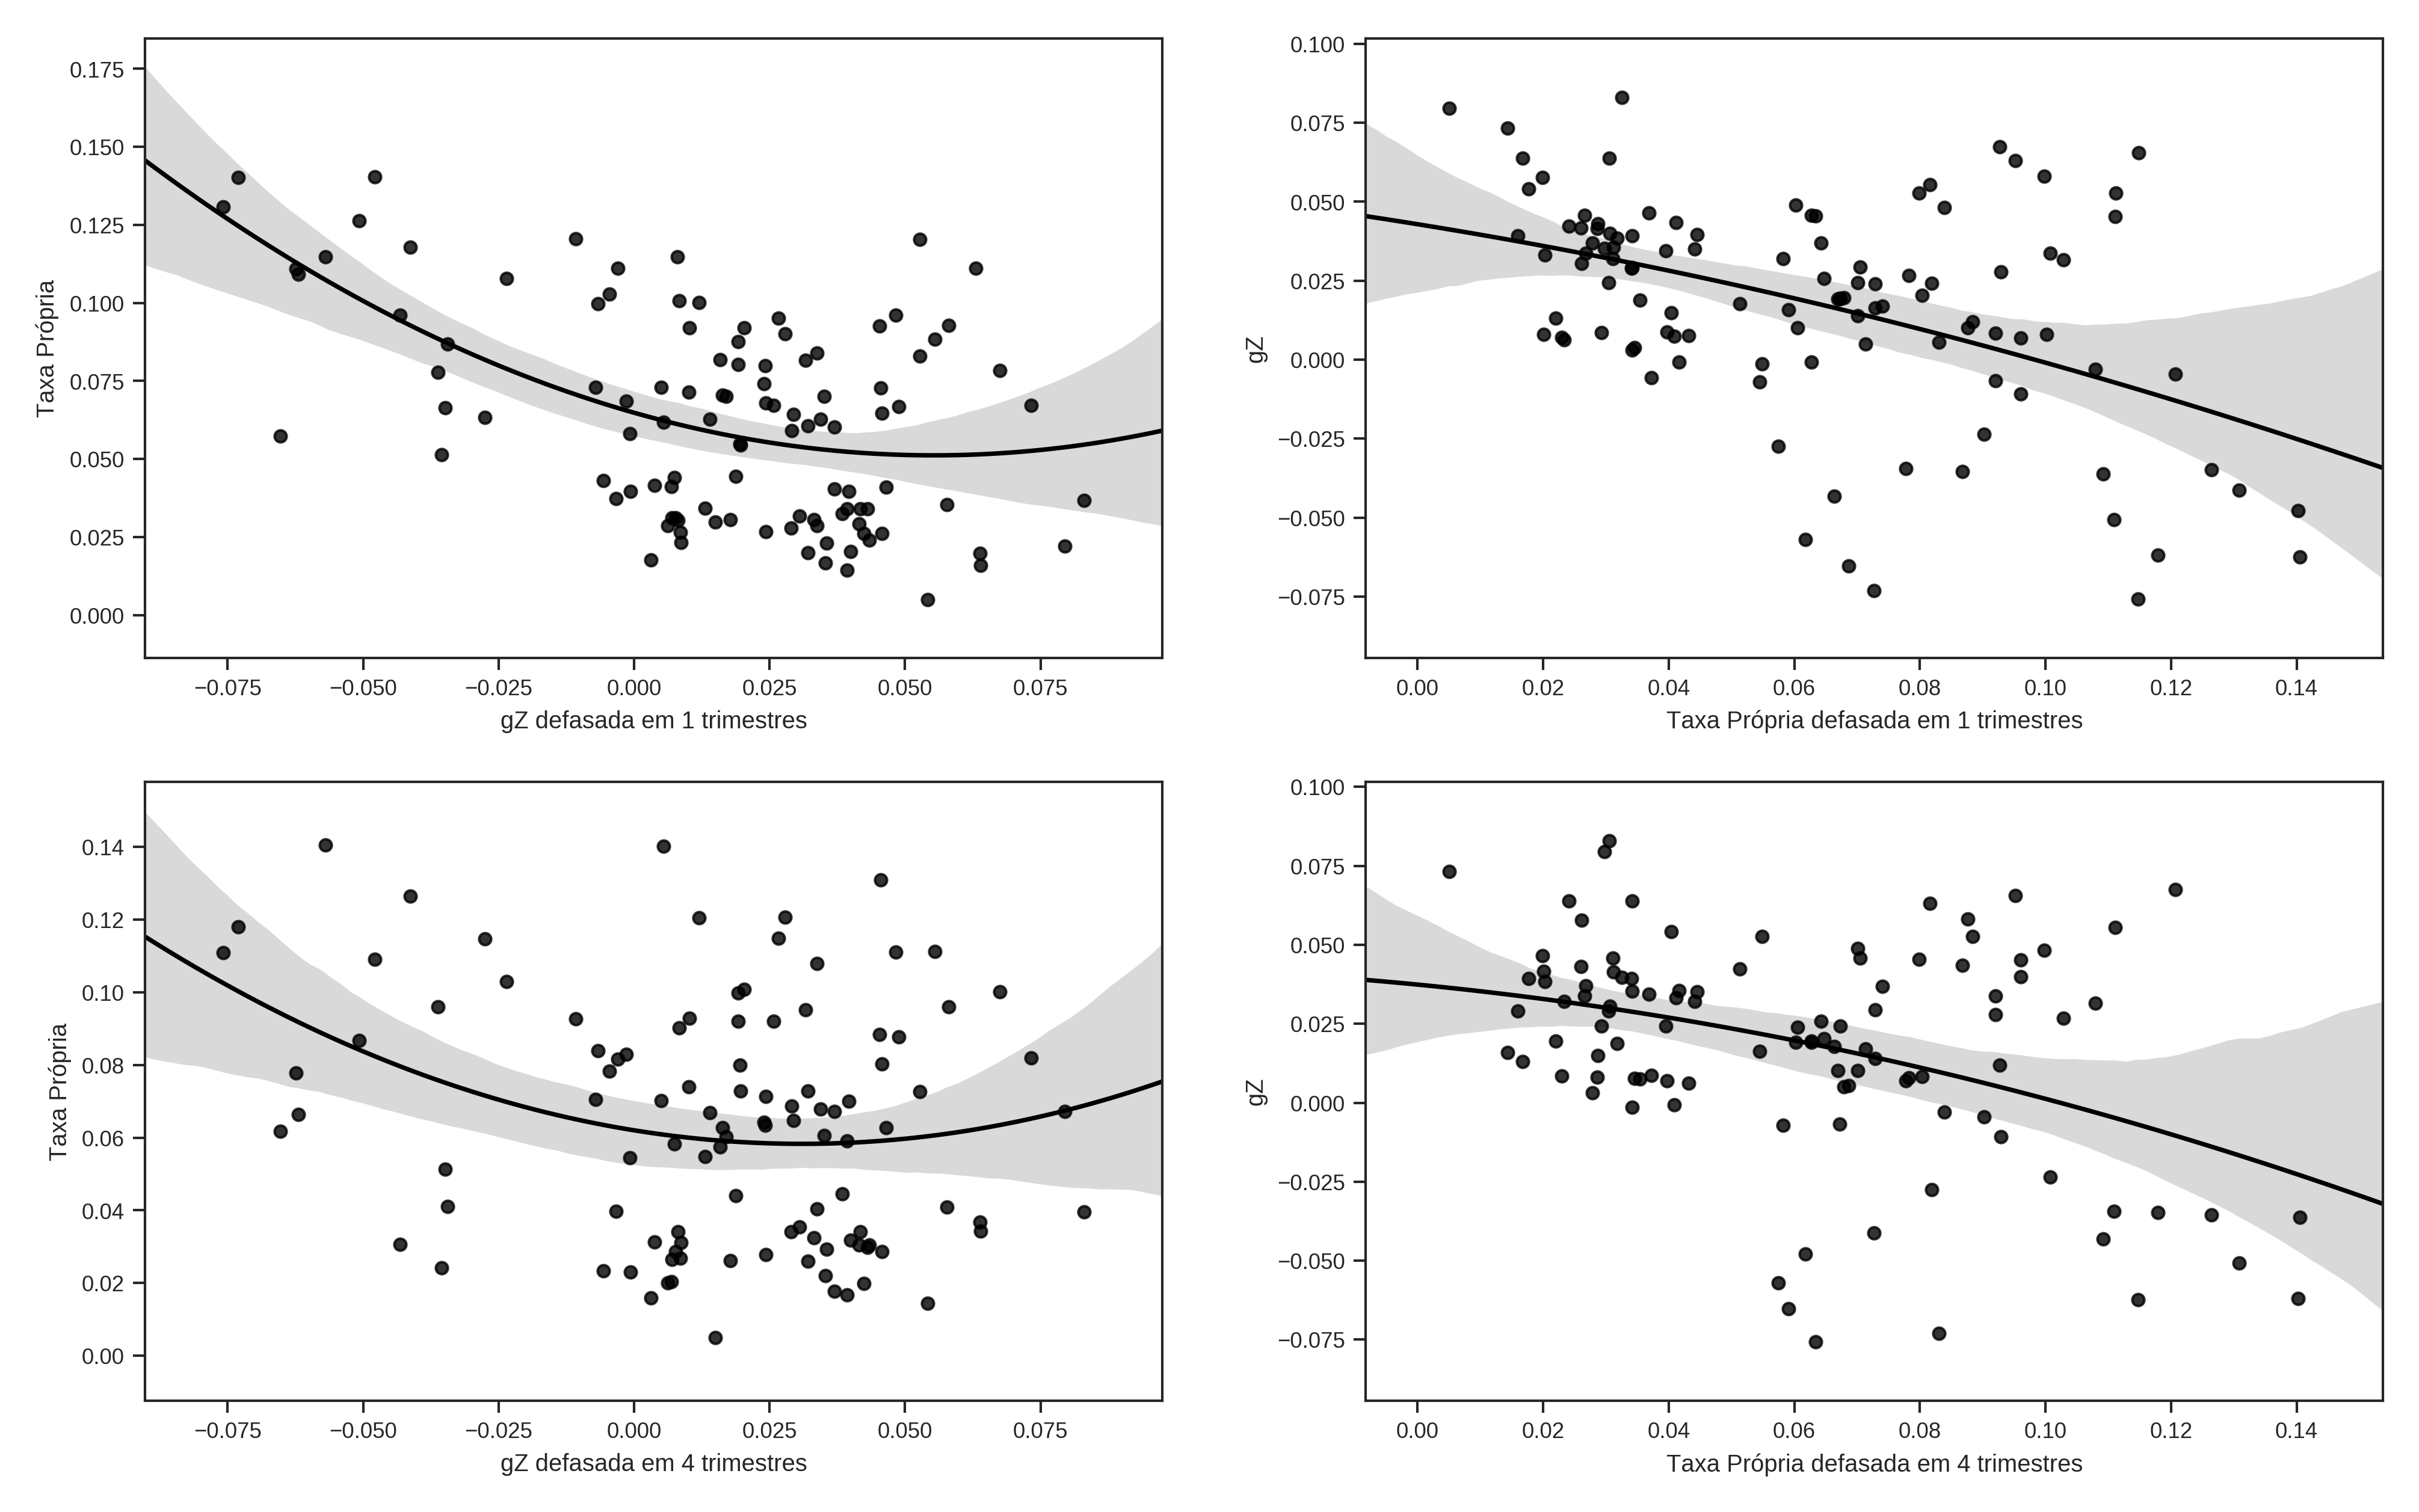
\includegraphics[width=\textwidth]{../../Modelo/SeriesTemporais/figs/VEC_Defasagens.png}
	\caption*{\textbf{Fonte:} Elaboração própria}
\end{figure}
%TODO Adicionar gráficos com defasagem 2


Feita esta contextualização teórica da escolha das defasagens, avança-se em direção a estimação do modelo. De modo a testar a capacidade explicativa da taxa própria para o investimento residencial, assume-se a seguinte relação de longo prazo tal como em \textcite{teixeira_crescimento_2015}:

\begin{equation}
g_{Z_t} = \phi_0 - \phi_1\cdot own_t
\end{equation}
que permite estimar um VEC nos seguintes termos:
\begin{equation}
\begin{cases}
\Delta own_t = \delta_{1} + \alpha_1(g_{Z_{t-1}} - \phi_0 + \phi_1\cdot own_{t-1}) + \sum^{N=4}_{i=1}\beta_{1,i}\cdot \Delta g_{Z_{t-i}} +
\sum^{N=4}_{i=1}\gamma_{1,i}\cdot \Delta own_{t-i} +\varepsilon_{t,1}
\\
\Delta g_{Z_{t}} = \delta_{2} + \alpha_2(g_{Z_{t-1}} - \phi_0 + \phi_1\cdot own_{t-1}) + \sum^{N=4}_{i=1}\beta_{2,i}\cdot \Delta g_{Z_{t-i}} +
\sum^{N=4}_{i=1}\gamma_{2,i}\cdot \Delta own_{t-i} +\varepsilon_{t,2}
\end{cases}
\end{equation}
em que $\delta_s$ indicam tendência linear nas respectivas séries em nível;
$\alpha_{is}$ são os coeficientes de correção de erro; 
$\beta_s$ e $\gamma_s$ são coeficientes associados as defasagens de  $g_Z$ e $own$ respectivamente e; $\varepsilon_s$ são os resíduos.
Seguindo a literatura do supermultiplicador sraffiano, os resultados esperados a serem testados são:
\begin{enumerate}
\item $\varepsilon \sim I(0)$: Estacionariedade dos resíduos indica que taxa própria e $g_Z$ são cointegrados, ou seja, apresentam uma dinâmica de longo prazo em comum;
\item $\alpha_1 = 0$: $own$ exogenamente fraca em relação ao $g_Z$;
\item $\alpha_2 < 0$: Taxa própria causa (no sentido de Granger) investimento residencial;
%TODO Checar sinal de alpha2
\item $\phi_1 > 0$: $gZ$ e Taxa própria apresentam uma dinâmica negativa no longo prazo;
\item $\phi_0 < 0$: Demanda por imóveis por motivos não-especulativos e associados a especificidades institucionais é estatisticamente significante e não-negativo;
\item $\gamma_{2,is} < 0$: Taxa própria afeta o investimento residencial negativamente no curto prazo;
\item $\beta_{1,is}$ = 0: Efeito do investimento de $g_Z$ sobre a taxa própria não é estatisticamente significante.
\end{enumerate}





\begin{figure}[H]
	\centering
	\caption{Inspeção dos resíduos da estimação}
	\label{residuos}
	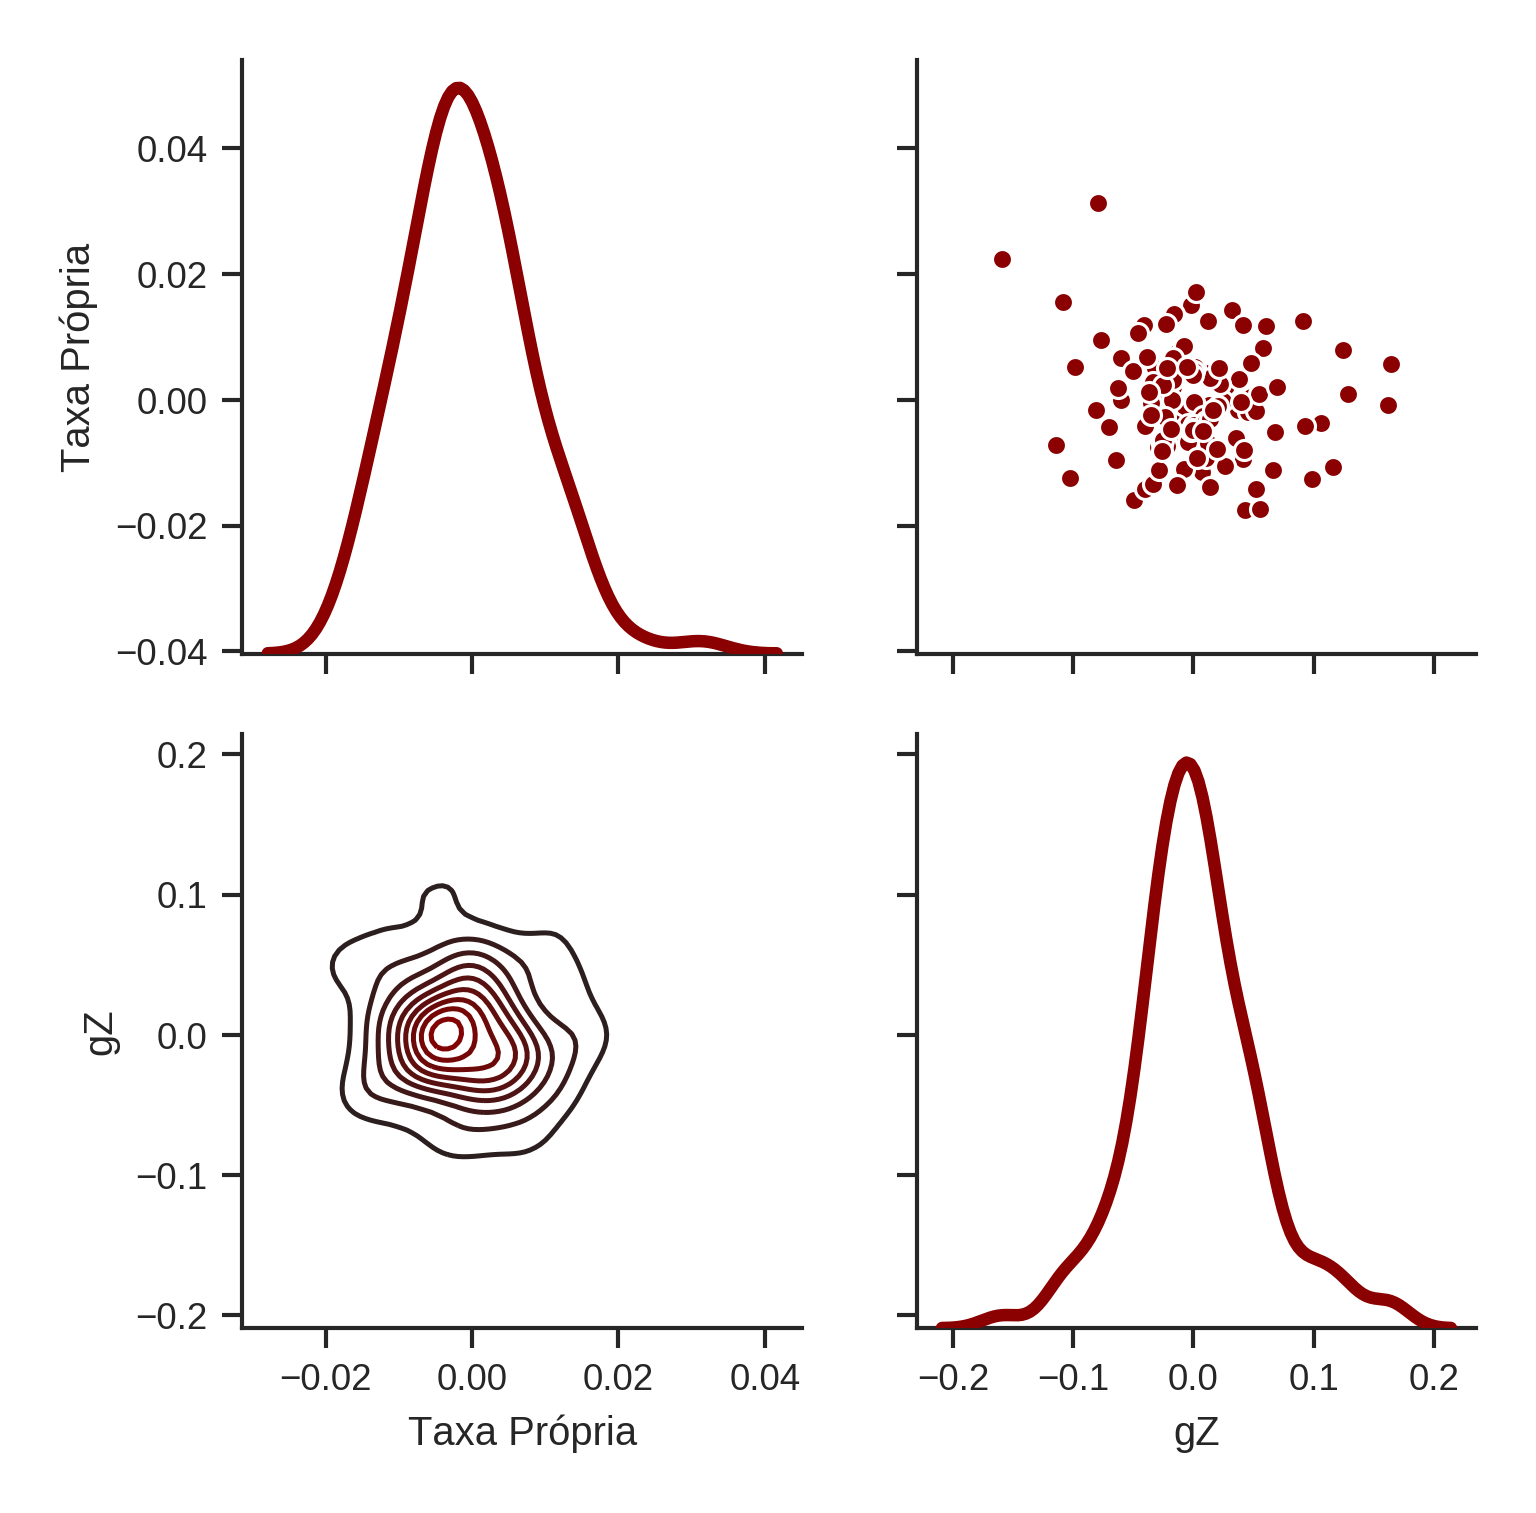
\includegraphics[height=.4\textheight]{../../Modelo/SeriesTemporais/figs/Residuos_4VECM.png}
	\caption*{\textbf{Fonte:} Elaboração própria}
\end{figure}

\begin{table}[htb]
\centering
	\caption{Parâmetros da estimação (VECM)}
\label{Estimacao}
\begin{threeparttable}
	\begin{tabular}{lcccccc}
		\hline \hline
		\textbf{Equação:} $own$ & \textbf{coef} & \textbf{std err} & \textbf{z} & \textbf{P$> |$z$|$} & \textbf{[0.025} & \textbf{0.975]}  \\
		\midrule
		\textbf{$\delta_{1}$}      &   -1.632e-05  &      4.4e-05     &    -0.371  &         0.710        &       -0.000    &     6.98e-05     \\
		\textbf{$\gamma_{1,1}$ ($L_1$ $own$)} &       0.0381  &        0.111     &     0.342  &         0.732        &       -0.180    &        0.256     \\
		\textbf{$\beta_{1,1}$ ($L_1 g_{I_h}$)}           &       0.0738  &        0.083     &     0.887  &         0.375        &       -0.089    &        0.237     \\
		\textbf{$\gamma_{1,2}$ ($L_2$ $own$)} &      -0.0032  &        0.110     &    -0.029  &         0.977        &       -0.218    &        0.212     \\
		\textbf{$\beta_{1,2}$ ($L_2 g_{I_h}$)}           &       0.1115  &        0.082     &     1.366  &         0.172        &       -0.048    &        0.272     \\
		\textbf{$\gamma_{1,3}$ ($L_3$ $own$)} &       0.0757  &        0.118     &     0.642  &         0.521        &       -0.156    &        0.307     \\
		\textbf{$\beta_{1,3}$ ($L_3 g_{I_h}$)}           &       0.1080  &        0.069     &     1.563  &         0.118        &       -0.027    &        0.243     \\
		\textbf{$\gamma_{1,4}$ ($L_4$ $own$)} &       0.2649  &        0.119     &     2.230  &         0.026$^{***}$        &        0.032    &        0.498     \\
		\textbf{$\beta_{1,4}$ ($L_4 g_{I_h}$)}           &      0.0583  &        0.054     &    1.089  &         0.276        &       -0.047    &       0.163     \\
		\midrule
		\textbf{Equação:} $g_{I_h}$ & \textbf{coef} & \textbf{std err} & \textbf{z} & \textbf{P$> |$z$|$} & \textbf{[0.025} & \textbf{0.975]}  \\
		\midrule
		\textbf{$\delta_{2}$}      &      -0.0003  &     6.96e-05     &    -3.848  &         0.000$^{***}$        &       -0.000    &       -0.000     \\
		\textbf{$\gamma_{2,1}$ ($L_1$ $own$)} &      -0.1747  &        0.176     &    -0.991  &         0.322        &       -0.520    &        0.171     \\
		\textbf{$\beta_{2,1}$ ($L_2 g_{I_h}$)}           &      -0.4203  &        0.132     &    -3.191  &         0.001$^{***}$        &       -0.678    &       -0.162     \\
		\textbf{$\gamma_{2,2}$ ($L_2$ $own$)} &      -0.9997  &        0.174     &    -5.752  &         0.000$^{***}$        &       -1.340    &       -0.659     \\
		\textbf{$\beta_{2,2}$ ($L_1 g_{I_h}$)}           &      -0.4596  &        0.129     &    -3.555  &         0.000$^{***}$        &       -0.713    &       -0.206     \\
		\textbf{$\gamma_{2,3}$ ($L_3$ $own$)} &      -0.5863  &        0.187     &    -3.137  &         0.002$^{***}$        &       -0.953    &       -0.220     \\
		\textbf{$\beta_{2,3}$ ($L_3 g_{I_h}$)}           &      -0.1991  &        0.109     &    -1.820  &         0.069*        &       -0.414    &        0.015     \\
		\textbf{$\gamma_{2,4}$ ($L_4$ $own$)} &      -0.5350  &        0.188     &    -2.844  &         0.004$^{***}$        &       -0.904    &       -0.166     \\
		\textbf{$\beta_{2,4}$ ($L_4 g_{I_h}$)}           &      -0.2444  &        0.085     &    -2.885  &         0.004$^{***}$        &       -0.411    &       -0.078     \\
		\midrule
		\textbf{Correção de Erro} & \textbf{coef} & \textbf{std err} & \textbf{z} & \textbf{P$> |$z$|$} & \textbf{[0.025} & \textbf{0.975]}  \\
		\midrule
		\textbf{$\alpha_1$} &      -0.0232  &        0.071     &    -0.328  &         0.743        &       -0.162    &        0.116     \\
		\textbf{$\alpha_2$} &      -0.4245  &        0.112     &    -3.784  &         0.000$^{***}$        &       -0.644    &       -0.205     \\
		\midrule
		\textbf{Relação de Cointegração} & \textbf{coef} & \textbf{std err} & \textbf{z} & \textbf{P$> |$z$|$} & \textbf{[0.025} & \textbf{0.975]}  \\
		\midrule
		\textbf{$\phi_{1,1}$} &       1.0000  &            0     &         0  &         0.000$^{***}$        &        1.000    &        1.000     \\
		\textbf{$\phi_{1,2}$} &       1.2835  &        0.149     &     8.599  &         0.000$^{***}$        &        0.991    &        1.576     \\
		\textbf{$\phi_0$}  &      -0.1131  &        0.009     &   -12.528  &         0.000$^{**}$       &       -0.131    &       -0.095     \\
		\hline
		\hline
	\end{tabular}
	%\caption{Det. terms outside the coint. relation & lagged endog. parameters for equation $own$}
\footnotesize{(*) Estatisticamente significante a 10\%; (**) Estatisticamente significante a 5\%; (***) Estatisticamente significante a 1\%.}
\end{threeparttable}
\caption*{\textbf{Fonte:} Elaboração própria}
\end{table}

%TODO Modificar tabela da estimação

Dito isso,  estima-se um VECM de ordem 4\footnote{Nota-se que tal defasagem, além de ser teoricamente justificada, também gera resíduos não heterocedásticos e sem correlação serial (ver tabela \ref{testes_resduos}).} cujos resíduos são apresentados no gráfico \ref{residuos} e resultados são expostos na tabela \ref{Estimacao}\footnote{Os resultados de todos os testes realizados bem como as rotinas utilizadas estão disponíveis sob solicitação.}.
Começando pela relação de cointegração, verifica-se que é estatisticamente significante para ambas as equações de modo que as variáveis partilham uma relação (negativa) de longo prazo, ou seja, são cointegradas (fundamentando 1 e 4).
Desse modo, a proposição de \textcite{teixeira_crescimento_2015} é corroborada por meio do coeficiente $\phi_1> 0$ e estatisticamente significante.
Além disso, os coeficientes $\gamma_{2,is}$ estimados são negativos seguindo os resultados esperados (6) do mesmo modo que a demanda por imóveis por motivos não-especulativos ($\phi_0$) é estatisticamente significante (resultado 5).
Adotando um nível de significância de 5\%, verifica-se que o parâmetro de correção de erro é estatisticamente significante apenas para a equação da taxa de crescimento do investimento residencial. Portanto, $own$ é exogenamente fraca em relação a $g_Z$ enquanto taxa própria Granger-causa $g_Z$, validando os resultado esperados (2) e (3).
Já as relações de curto prazo entre taxa própria e $g_Z$ (capturadas por $\beta_{1,is}$) não são estatisticamente significantes a 5\% \footnote{O resultado esperado (7) também pode ser confirmado a partir da inspeção da tabela \ref{Estimacao} em que apenas a quarta defasagem da taxa própria é estatisticamente significante nesta equação.}. Em resumo, os resultados obtidos estão em linha com os esperados. 

Uma forma de verificar a capacidade explicativa da taxa própria para $g_Z$ é por meio da decomposição da variância da previsão (FEVD) como no gráfico \ref{fevd}\footnote{Também é importante destacar que dado o número de variáveis (duas), a ordenação de Choleski é suficiente para analisar a função resposta ao impulso uma vez que gera uma matriz semelhante a de um VECM estrutural. 
}. Verifica-se que desde o primeiro trimestre a taxa própria contribui para $g_Z$ enquanto o inverso não é válido. Adicionalmente, é notável que tal contribuição é crescente e maior que 50\% para além do 3º trimestre. Portanto, a taxa própria é explicada principalmente por ela mesma e explica $g_Z$ consideravelmente.

\begin{figure}[htb]
	\centering
	\caption{Decomposição da variância da previsão}
	\label{fevd}
	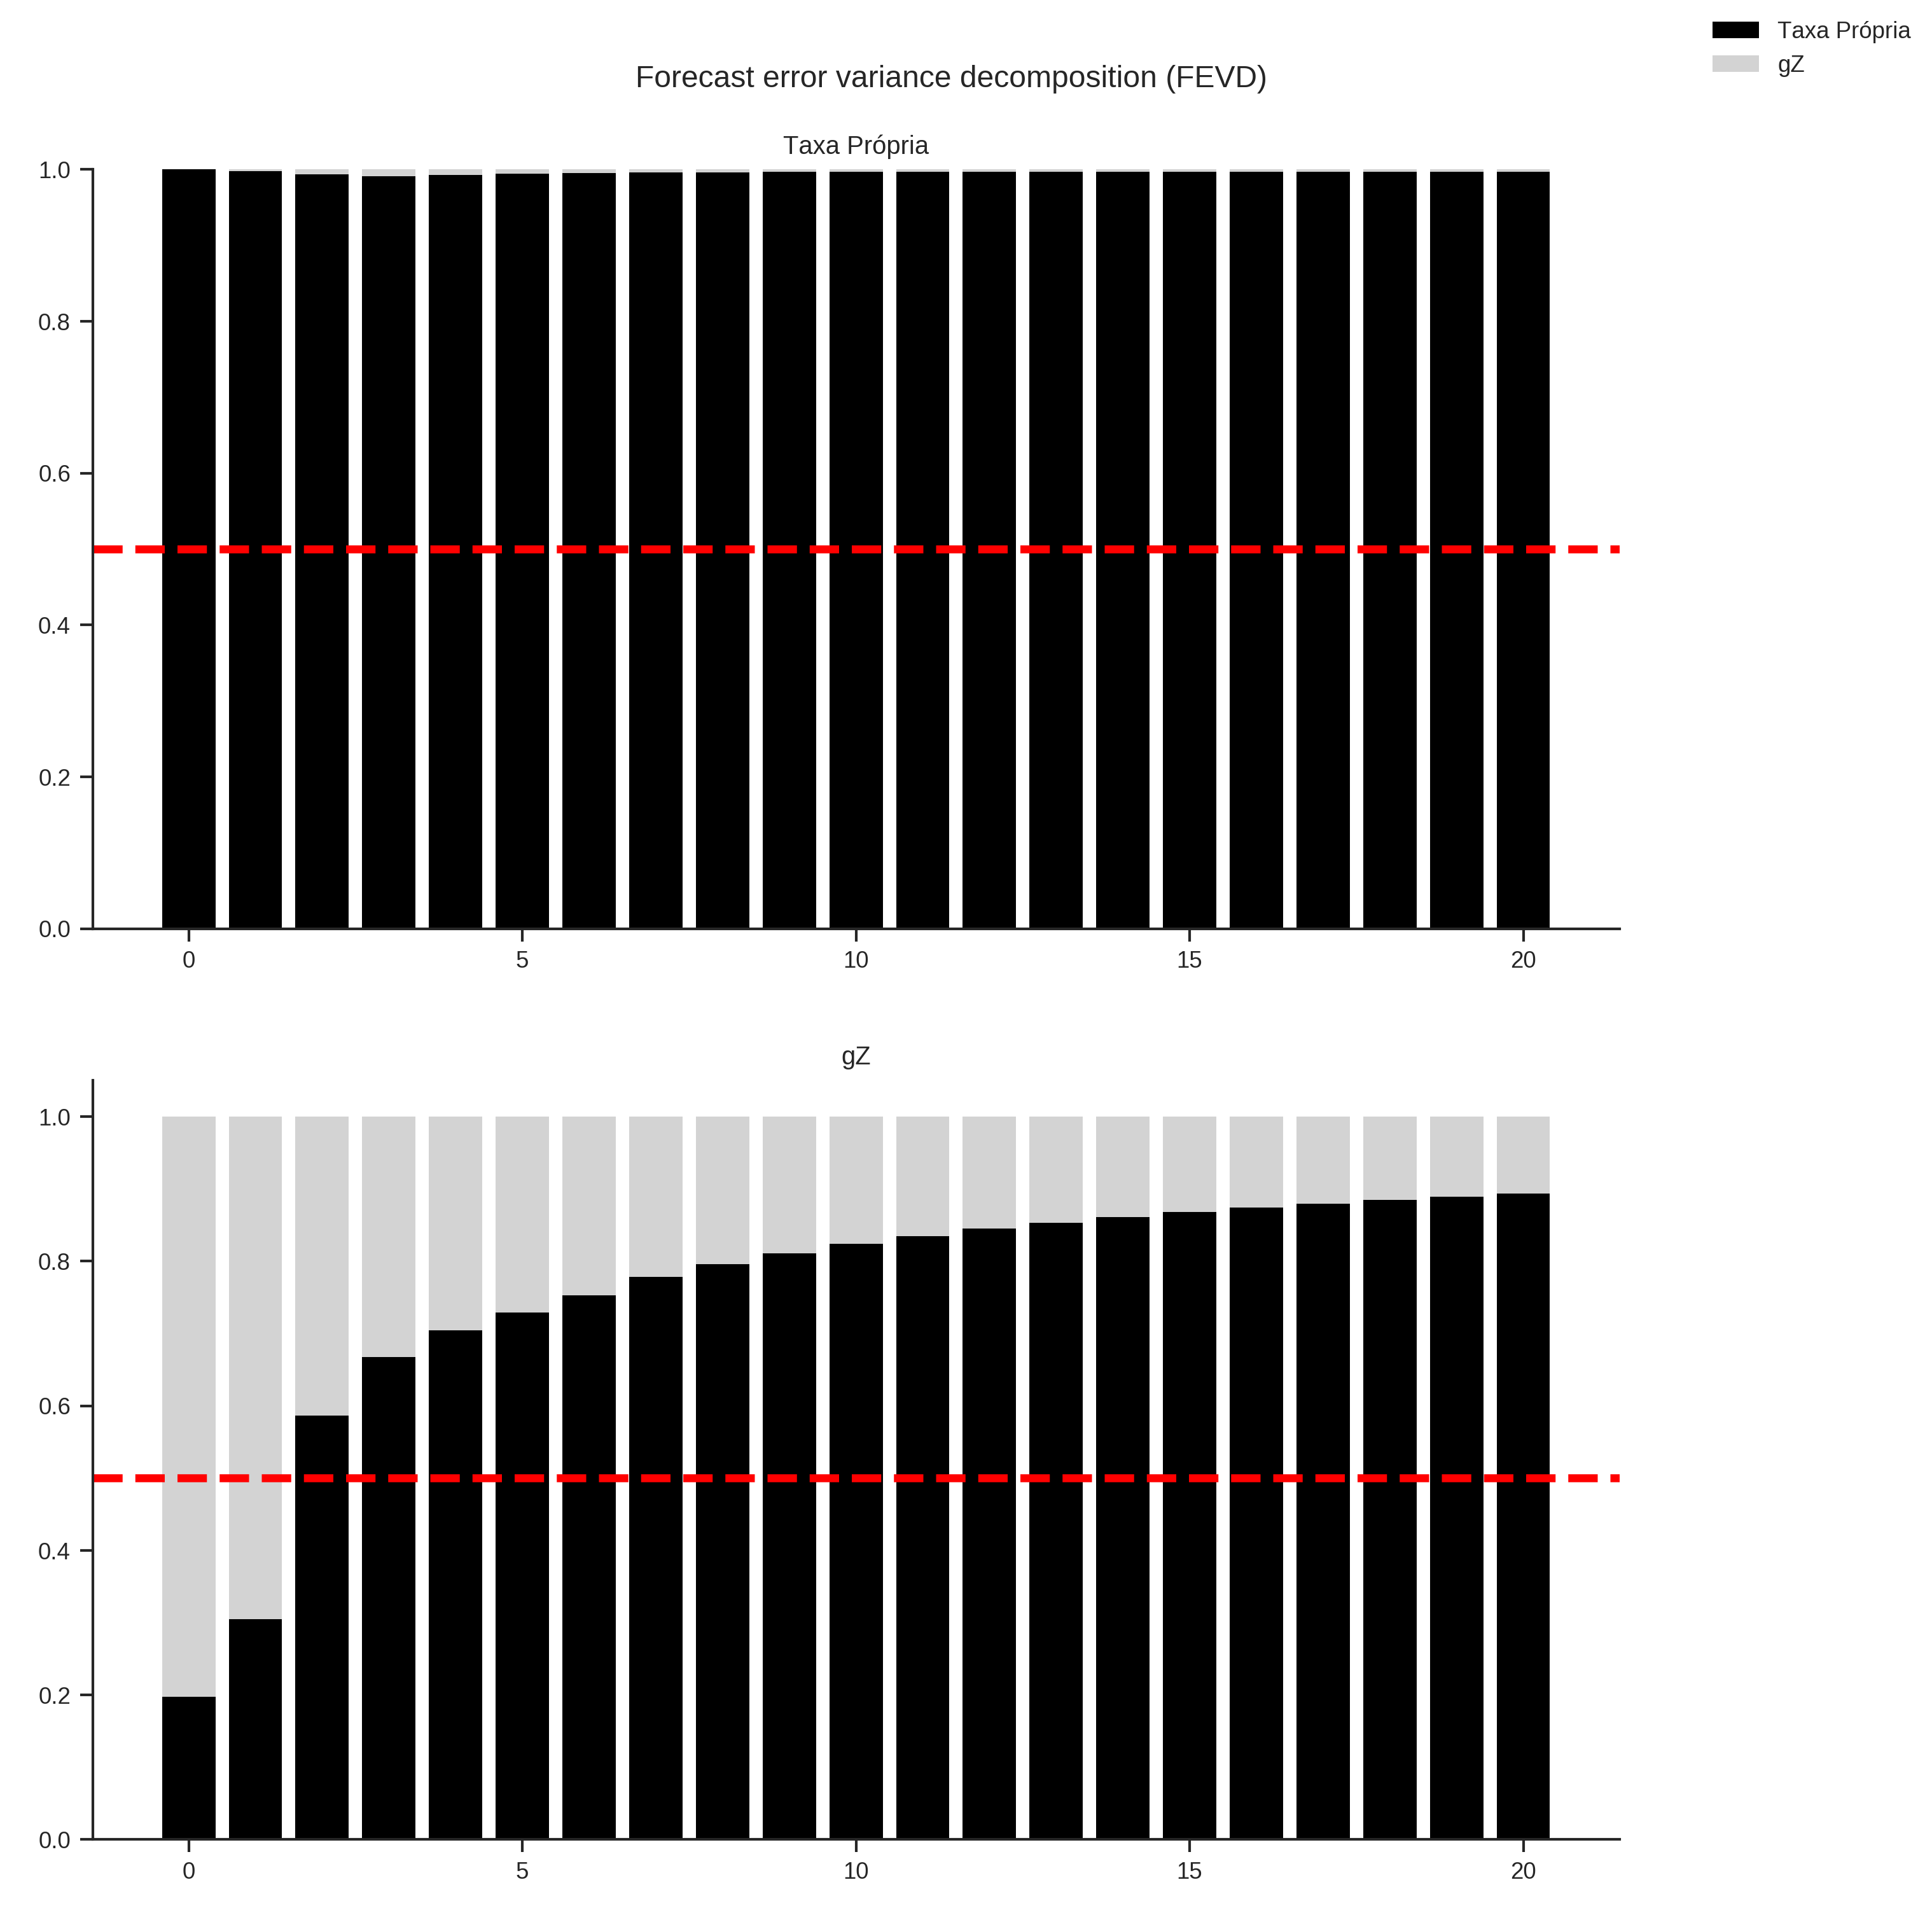
\includegraphics[width=\textwidth]{../../Modelo/SeriesTemporais/figs/FEVD_VECMpython_TxPropria.png}
	\caption*{\textbf{Fonte:} Elaboração própria}
\end{figure}


Adiante, é apresentado o gráfico da função impulso resposta ortogonalizada --- grosso modo, as conclusões da FEVD se estendem também para os choques --- em que são avaliados os impactos no aumento de um desvio-padrão em uma das variáveis endógenas no primeiro período apenas.
%TODO Checar
A partir deste gráfico, verifica-se que o sistema é estável uma vez que os efeitos do aumento de $g_Z$ sobre $g_Z$ é amortecido ao longo do tempo enquanto os efeitos da taxa própria sobre a ela mesma são persistentes mas não explosivos.
Já os efeitos de $g_Z$ sobre a taxa própria é nulo uma vez que o intervalo de confiança sempre abrange o zero. Por fim, e este é o resultado relevante, dados os objetivos, é o efeito negativo considerável e duradouro da taxa própria sobre $g_Z$, confirmando a tese de \textcite{teixeira_crescimento_2015}.
Em resumo, as funções resposta ao impulso indicam que o aumento da taxa de juros das hipotecas (aumento na Taxa Própria) impacta negativamente na taxa de crescimento residencial enquanto o aumento da inflação de ativos implica no inverso. 
%alinhado com os resultados de \textcite{huang_is_2018} para o longo prazo.
%podendo estar associado aos gastos com aprimoramento residencial uma vez encerradas as construções (também contabilizado como investimento residencial).


\begin{figure}[H]
	\centering
	\caption{Função impulso resposta ortogonalizada}
	\label{fevd}
	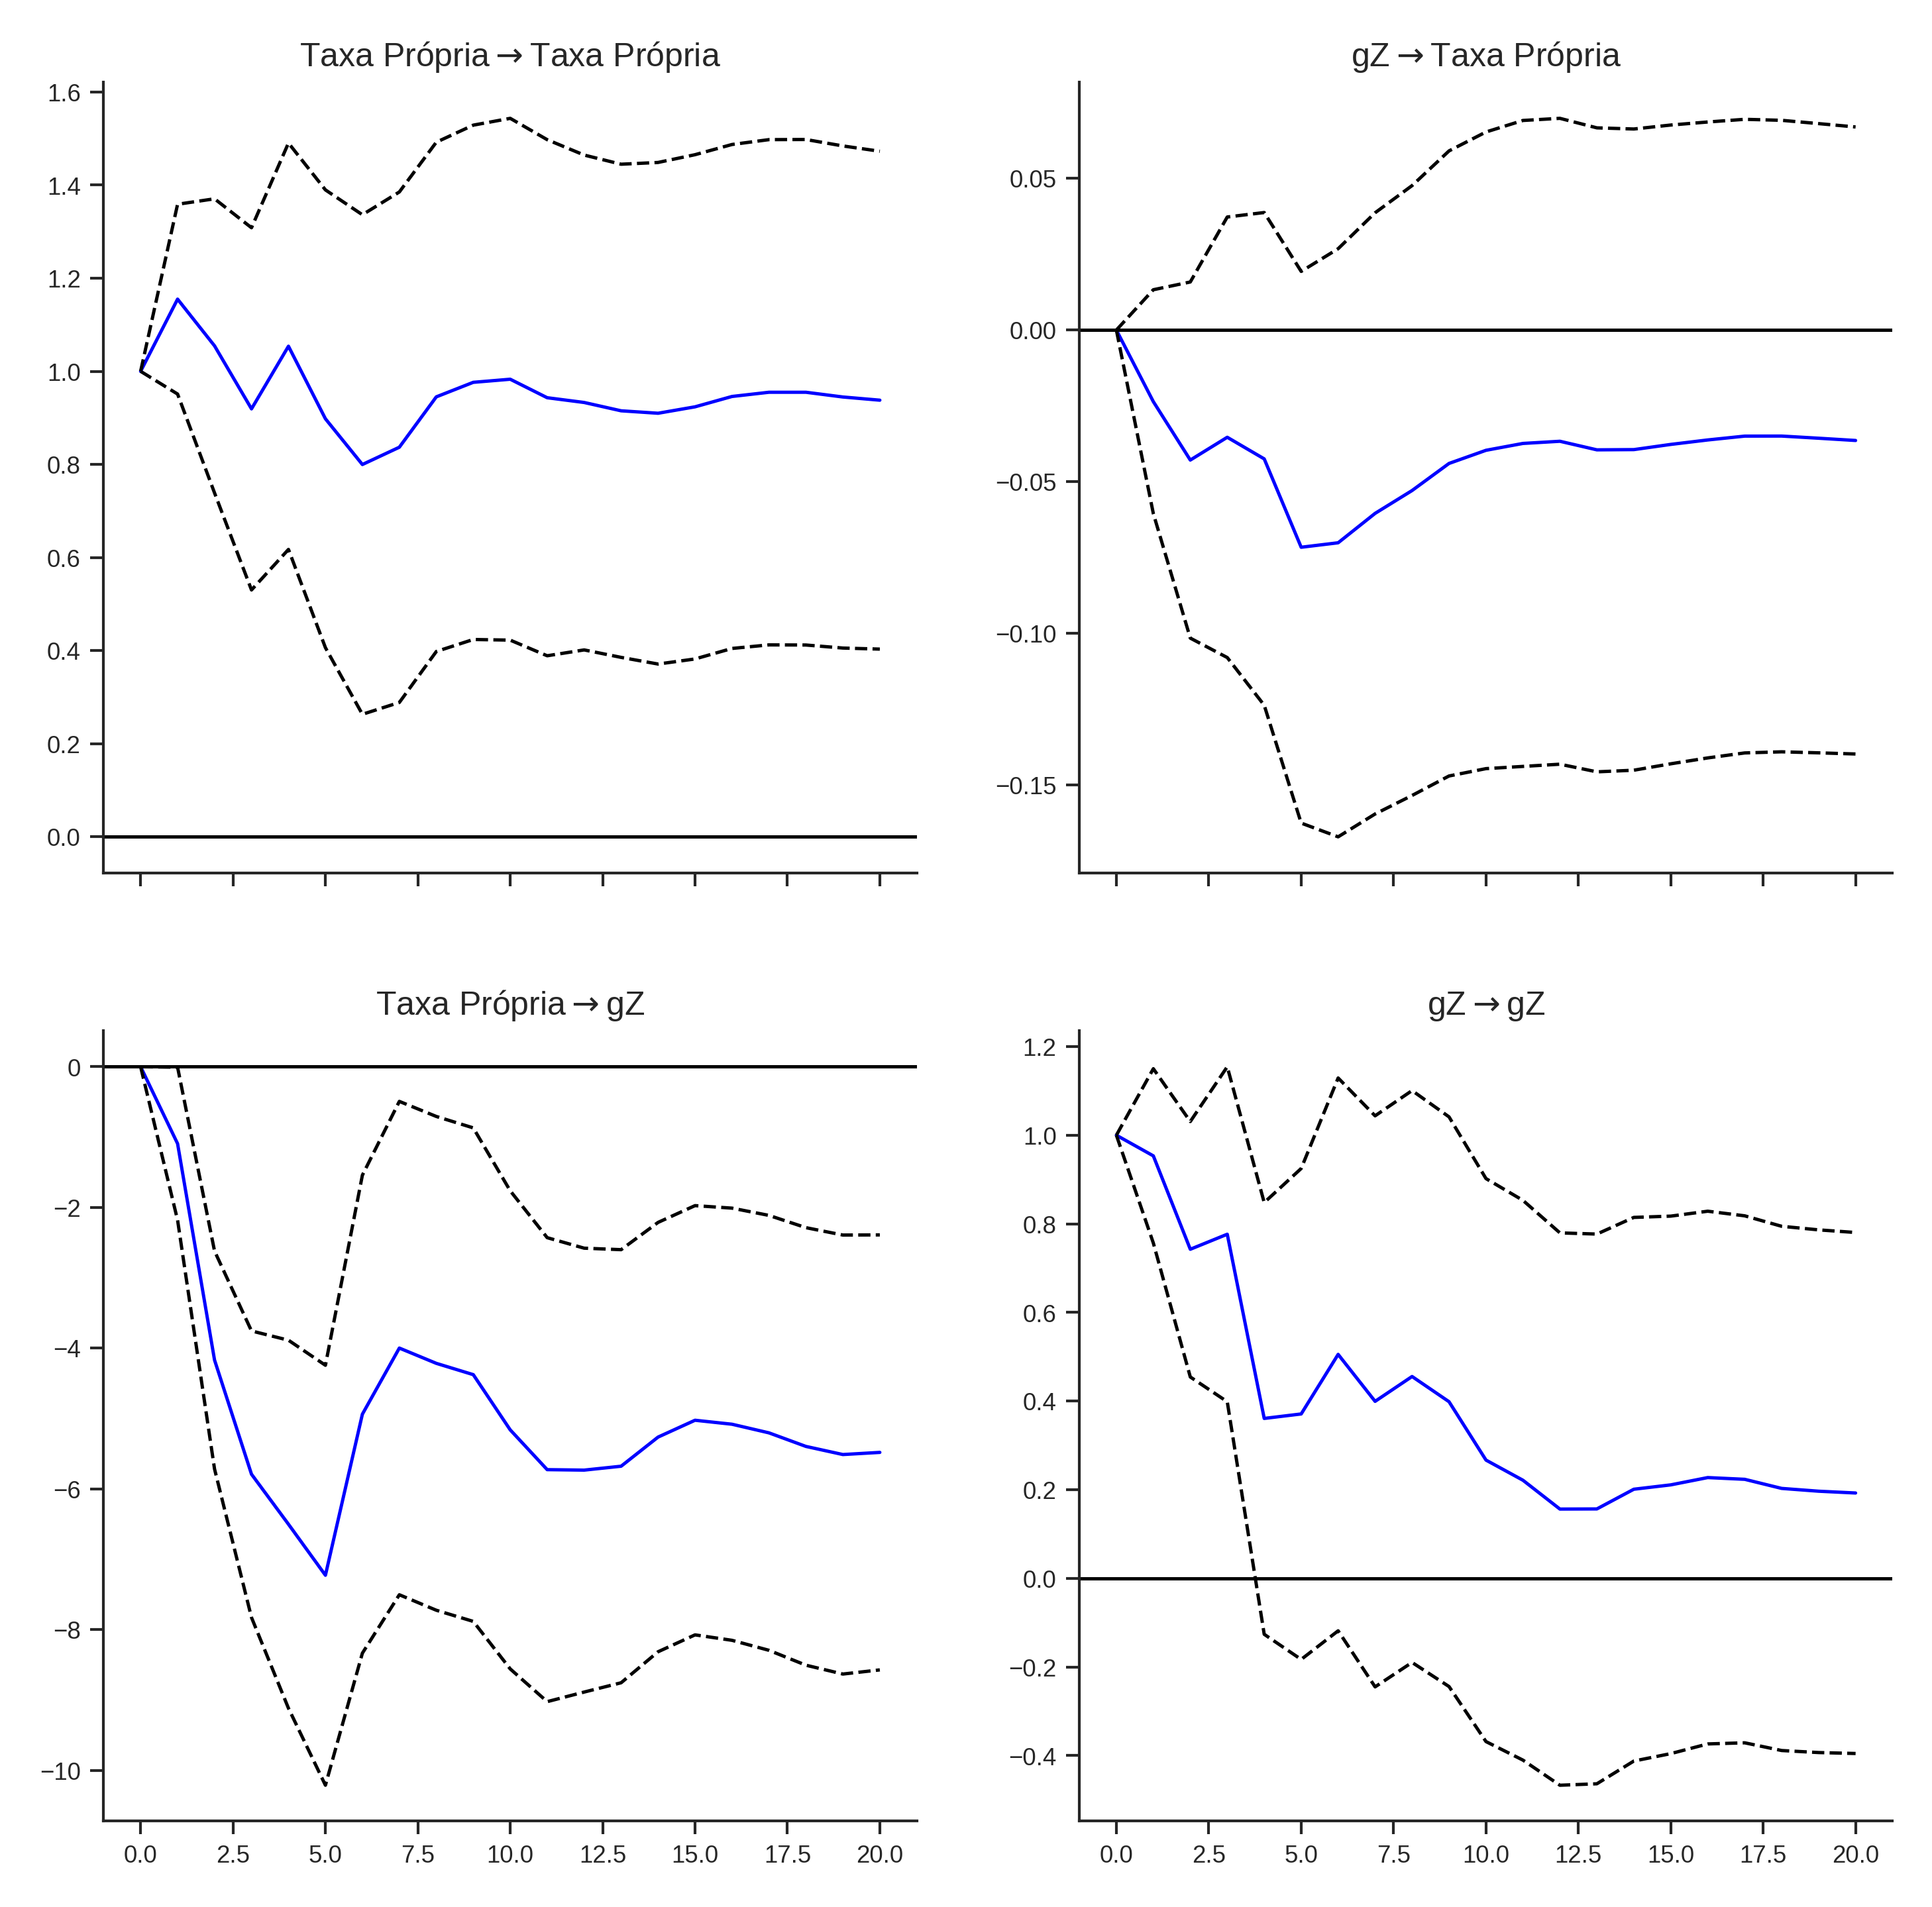
\includegraphics[width=\textwidth]{../../Modelo/SeriesTemporais/figs/Impulso_VECM.png}
	\caption*{\textbf{Fonte:} Elaboração própria}
\end{figure}

Dos resultados apresentados acima, verifica-se que a taxa própria de juros dos imóveis tem uma capacidade explicativa significativa. Vale destacar que apesar de amplitude das defasagens selecionadas, o modelo estimado é bastante parcimonioso em termos das variáveis utilizadas. Desse modo, considerando o grau de parcimônia e a robustez dos resultados, conclui-se que é um modelo satisfatório para explicar a taxa de crescimento do investimento residencial. 
%Diante da qualidade do ajuste, o gráfico \ref{previsao} apresenta a previsão do modelo 4 passos a frente. 
%Avaliando o últimos resultados disponíveis das contas nacionais e estimativas da taxa própria, verifica-se uma previsão satisfatória uma vez que tanto $g_Z$ reduz quanto a taxa própria aumenta.

\begin{comment}
\begin{figure}[H]
	\centering
	\caption{Previsão 4 passos a frente}
	\label{previsao}
	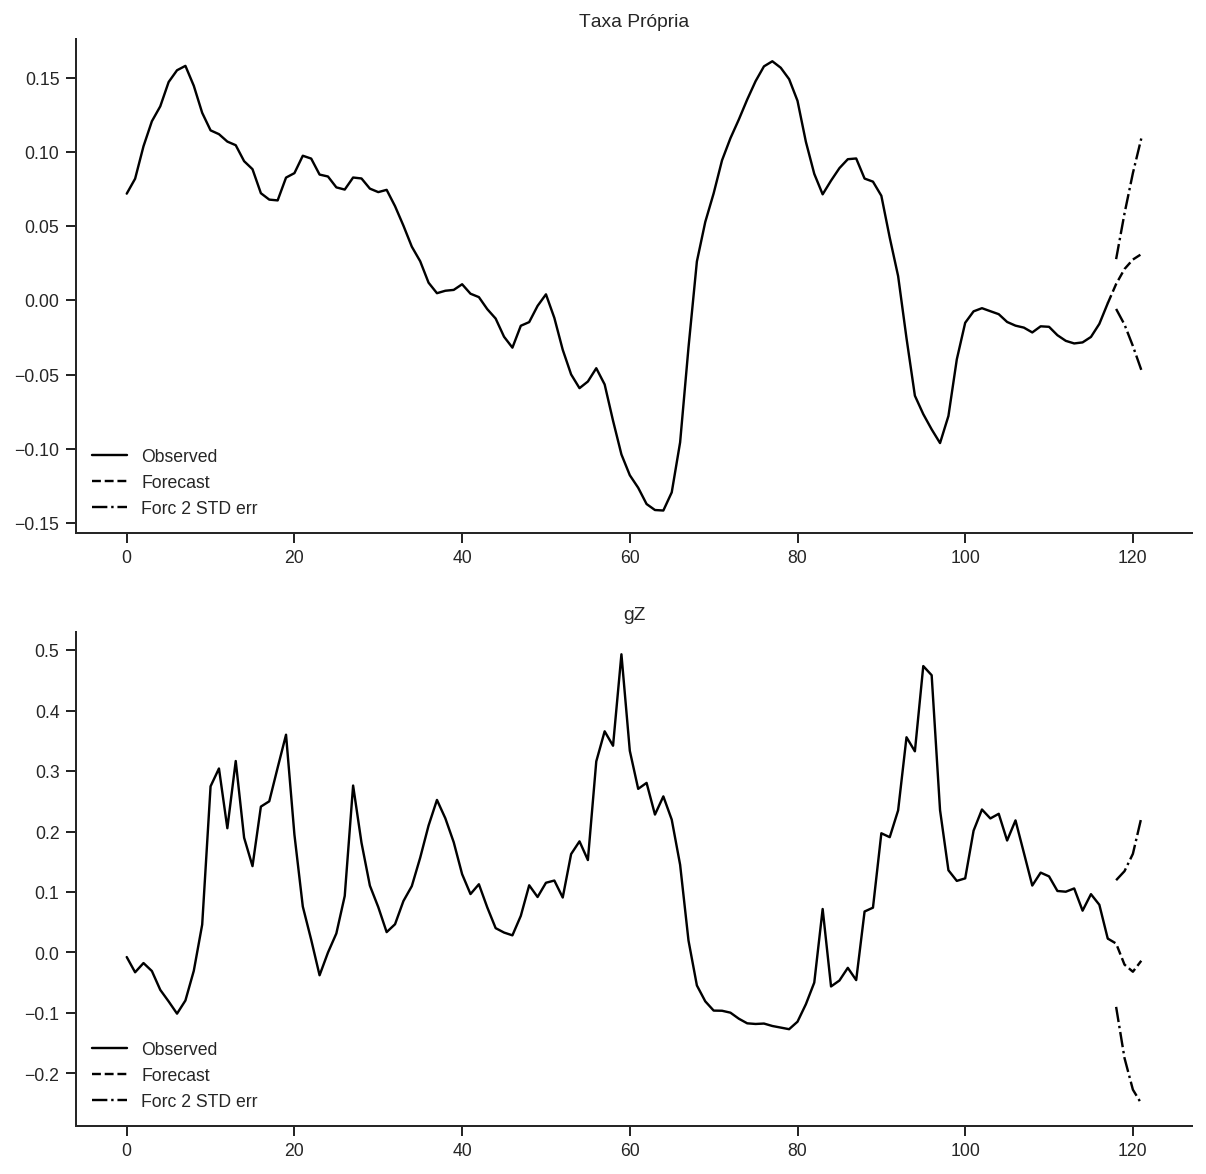
\includegraphics[width=\textwidth]{Fatos_Estilizados/Figs/Previsao_VECM.png}
	\caption*{\textbf{Fonte:} Elaboração própria}
\end{figure}


\begin{center}
\begin{table}[H]
\centering
\caption{Parâmetros para a equação da Taxa Própria}
\begin{tabular}{lccclcc}
\toprule
\textbf{Equação:} Taxa própria & \textbf{coef} & \textbf{std err} & \textbf{z} & \textbf{P$> |$z$|$} & \textbf{[0.025} & \textbf{0.975]}  \\
\midrule
\textbf{$L^1 $ Taxa Própria} &       0.9320  &        0.089     &    10.511  &         0.000***        &        0.758    &        1.106     \\
\textbf{$L^1 $ gZ}           &      -0.0545  &        0.014     &    -3.786  &         0.000***        &       -0.083    &       -0.026     \\
\textbf{$L^2 $ Taxa Própria} &      -0.2810  &        0.122     &    -2.305  &         0.021**        &       -0.520    &       -0.042     \\
\textbf{$L^2 $ gZ}           &       0.0040  &        0.013     &     0.309  &         0.758        &       -0.021    &        0.029     \\
\textbf{$L^3 $ Taxa Própria} &       0.0043  &        0.127     &     0.034  &         0.973        &       -0.245    &        0.253     \\
\textbf{$L^3 $ gZ}           &      -0.0132  &        0.012     &    -1.058  &         0.290        &       -0.038    &        0.011     \\
\textbf{$L^4 $ Taxa Própria} &      -0.0626  &        0.126     &    -0.497  &         0.619        &       -0.309    &        0.184     \\
\textbf{$L^4 $ gZ}           &      -0.0030  &        0.012     &    -0.242  &         0.809        &       -0.027    &        0.021     \\
\textbf{$L^5 $ Taxa Própria} &       0.0144  &        0.093     &     0.156  &         0.876        &       -0.167    &        0.196     \\
\textbf{EC1} &      -0.0099  &        0.007     &    -1.339  &         0.181        &       -0.024    &        0.005     \\
\textbf{$\beta_1$ } &       1.0000  &            0     &         0  &         0.000***        &        1.000    &        1.000     \\\bottomrule
\end{tabular}
\caption*{\textbf{Fonte:} Elaboração própria}
\end{table}
\end{center}

\begin{table}[H]
\begin{center}
\caption{Parâmetros para a equação da $g_Z$}	
\begin{tabular}{lccclcc}
\toprule
\textbf{Equação:} $g_Z$ & \textbf{coef} & \textbf{std err} & \textbf{z} & \textbf{P$> |$z$|$} & \textbf{[0.025} & \textbf{0.975]}  \\
\midrule
\textbf{$L^1 $ Taxa Própria} &      -0.8392  &        0.553     &    -1.517  &         0.129        &       -1.924    &        0.245     \\
\textbf{$L^1 $ gZ}           &       0.1290  &        0.090     &     1.435  &         0.151        &       -0.047    &        0.305     \\
\textbf{$L^2 $ Taxa Própria} &      -1.6629  &        0.761     &    -2.186  &         0.029**        &       -3.154    &       -0.172     \\
\textbf{$L^2 $ gZ}           &      -0.0663  &        0.081     &    -0.817  &         0.414        &       -0.225    &        0.093     \\
\textbf{$L^3 $ Taxa Própria} &       1.5635  &        0.793     &     1.972  &         0.049**        &        0.009    &        3.118     \\
\textbf{$L^3 $ gZ}           &       0.1092  &        0.078     &     1.407  &         0.159        &       -0.043    &        0.261     \\
\textbf{$L^4 $ Taxa Própria} &      -0.5929  &        0.785     &    -0.755  &         0.450        &       -2.132    &        0.946     \\
\textbf{$L^4 $ gZ}           &      -0.4590  &        0.078     &    -5.895  &         0.000***        &       -0.612    &       -0.306     \\
\textbf{$L^5 $ Taxa Própria} &      -0.3158  &        0.577     &    -0.547  &         0.584        &       -1.447    &        0.816     \\
\textbf{$L^5 $ gZ}           &       0.0265  &        0.089     &     0.299  &         0.765        &       -0.147    &        0.200     \\
\textbf{EC1} &       0.1388  &        0.046     &     3.021  &         0.003**        &        0.049    &        0.229     \\
\textbf{$\beta_2$ } &      -0.4833  &        0.230     &    -2.099  &         0.036**        &       -0.934    &       -0.032     \\\bottomrule
\end{tabular}
\caption*{\textbf{Fonte:} Elaboração própria}
\end{center}
\end{table}

\end{comment}

\section{Concluding Remarks}\label{sec:Conclusion}

In this article, we present a residential investment growth rate specification compatible with the Srrafian supermultiplier model.
To do so, we estimate a bi-dimension VEC evaluate \textcite{teixeira_crescimento_2015}
proposal. 
We report: 
	(i) Houses' own interest rate ($own$) and residential investment growth rate ($g_{I_h}$) share a common long-run trend;
	(ii) $g_{I_h}$ effects over $own$ are negligible and; 
	(iii) own interest rate has a negative effect on $g_{I_h}$ and is its main determinant (see Figure \ref{fevd}).
Besides being parsimonious, our estimations does not show residuals serial autocorrelation and heteroscedasticity. Thus, our results are quite satisfactory.

It remains to contrast our findings with those obtained by \textcite{arestis_residential_2015}.
It worth remembering that one of the authors' hypotheses is that residential investment depends on disposable income (is induced expenditure).
However, the authors themselves find that such results are not statistically significant for the US. Therefore, we can compare this result with our model.
Despite the differences, some results of the model are in line with those of \textcite{arestis_residential_2015}.
Among them, house prices relevance in determining residential investment dynamics for the US.
However, they report insignificant coefficients for mortgages nominal interest rate, that is, the opposite conclusion of our model.

In conclusion,  we report lack of work analyzing residential investment in a Sraffian supermultiplier-friendly framework in the macroeconometric literature.
Our estimation supports houses' own interest rate relevance in describing residential investment growth rate for the US as depicted by \textcite{teixeira_crescimento_2015}.
Thus, our  proposal differs from the usual empirical literature by:
	(i) considering housing as a non-capacity creating autonomous expenditure;
	(ii) reporting that mortgage interest rates are relevant to describe long-run residential investment dynamics; and notably 
	(iii) including asset bubble through houses own interest rate.



\section*{Acknowledgments}

\noindent We are grateful to  Rosângela Ballini, Carolina Baltar, Júlia Braga, Ítalo Pedrosa, Cecon/Unicamp and UFRJ Macroeconomic discussion groups for useful comments and suggestions on earlier drafts of this article. All remaining errors are, of course, our own.

\section*{Disclosure statement}

\noindent No potential conflict of interest was reported by the authors.


\printbibliography{}

\begin{appendix}
	\section{Numerical Appendix}\label{Appen:A}
\end{appendix}

\end{document}